\documentclass{article}
\usepackage{graphicx} % Required for inserting images
\usepackage{amssymb, amsthm}
\usepackage[fleqn]{amsmath}
\newcommand{\dkreis}[1]{%
	\tikz[baseline=(char.base)]{
		\node[shape=circle,draw,line width=1pt,inner sep=1.5pt] 
		(char) {\bfseries #1};
	}%
}
\setlength{\mathindent}{0.5cm}
\makeatletter
\renewcommand\tagform@[1]{}
\makeatother
\usepackage{float}
\usepackage[a4paper, margin=2.5cm]{geometry}
\usepackage{wrapfig}
\usepackage{multicol}
\usepackage{pgfplots}
\pgfplotsset{compat=1.18}
\usepgfplotslibrary{statistics}
\usetikzlibrary{circuits.ee.IEC}
\usepackage{enumitem}
\usepackage{setspace}
\setstretch{1.2}
\usepackage[font=small, labelfont=bf, justification=centering, singlelinecheck=false]{caption}
\usepackage[T1]{fontenc}
\usepackage[utf8]{inputenc}
\usepackage[ngerman]{babel}
\usepackage{csquotes}
\usepackage{tikz, siunitx}
\usepackage[most]{tcolorbox}
\usetikzlibrary{decorations.pathmorphing,arrows.meta}
\sisetup{
	per-mode = fraction,
	separate-uncertainty = true
}


\title{Elektromagnetismus - Tepe}
\author{Arthur Thiele}
\date{Q1-Q2}

\begin{document}
	
	\maketitle
	\newpage 
	
	\section{Der {\O}rsted-Versuch}
	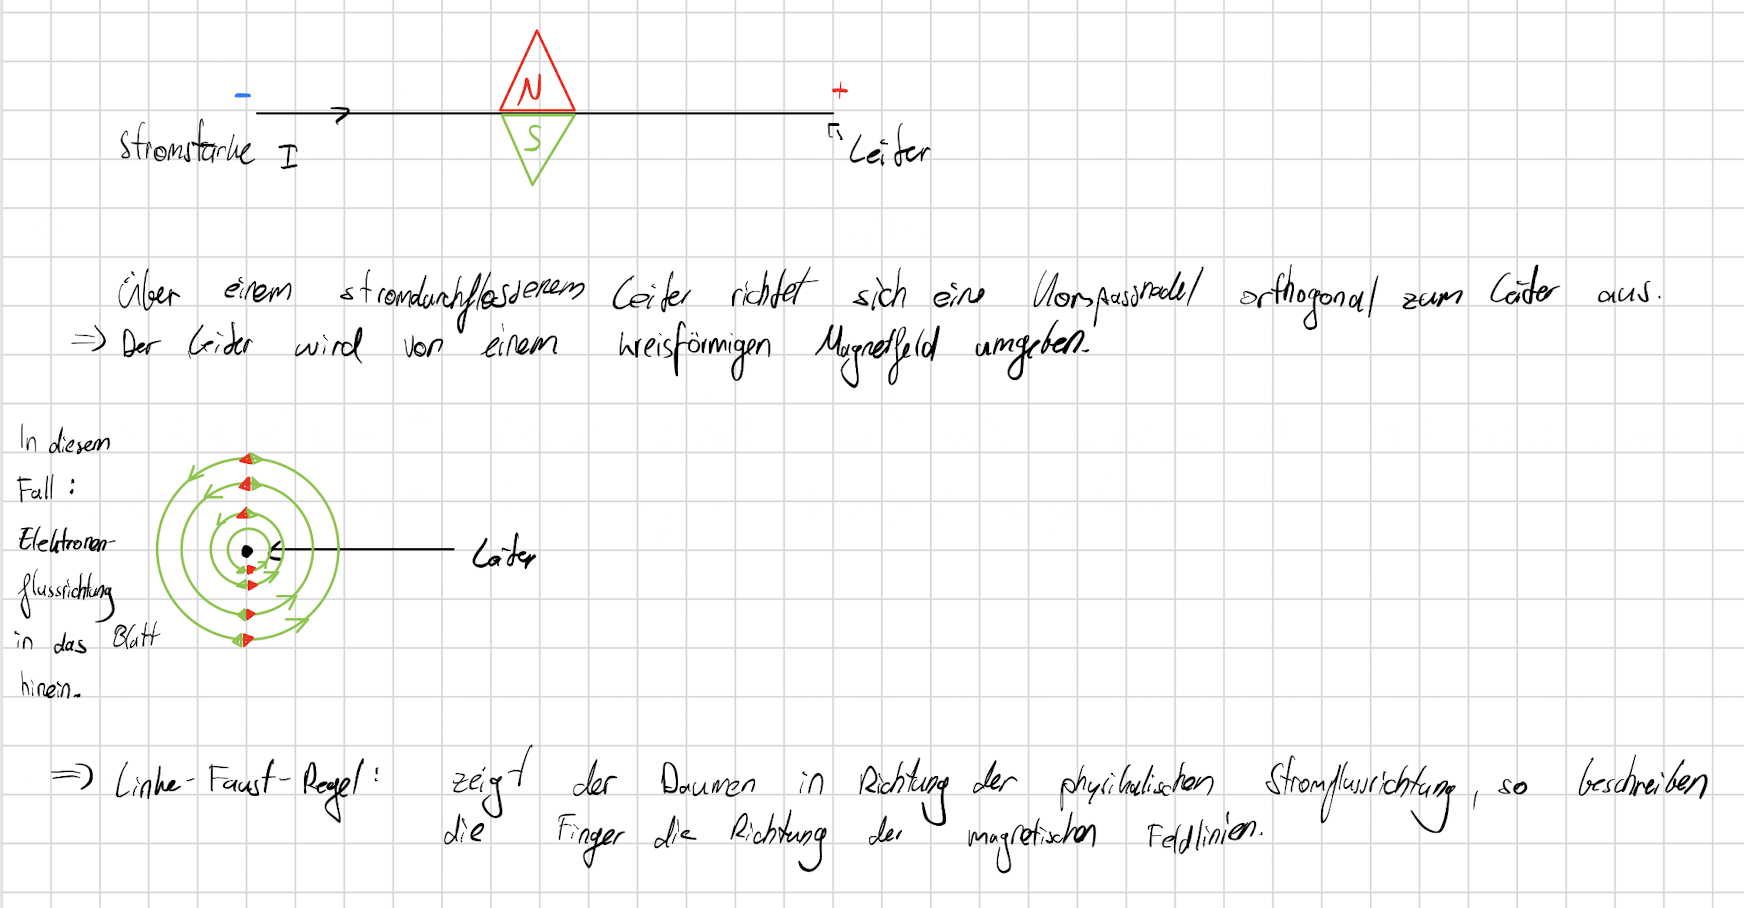
\includegraphics[width=\textwidth]{Images/Orsted Versuch.png}
	\newpage
	\section{Das Magnetfeld einer stromdurchflossenen Spule}
	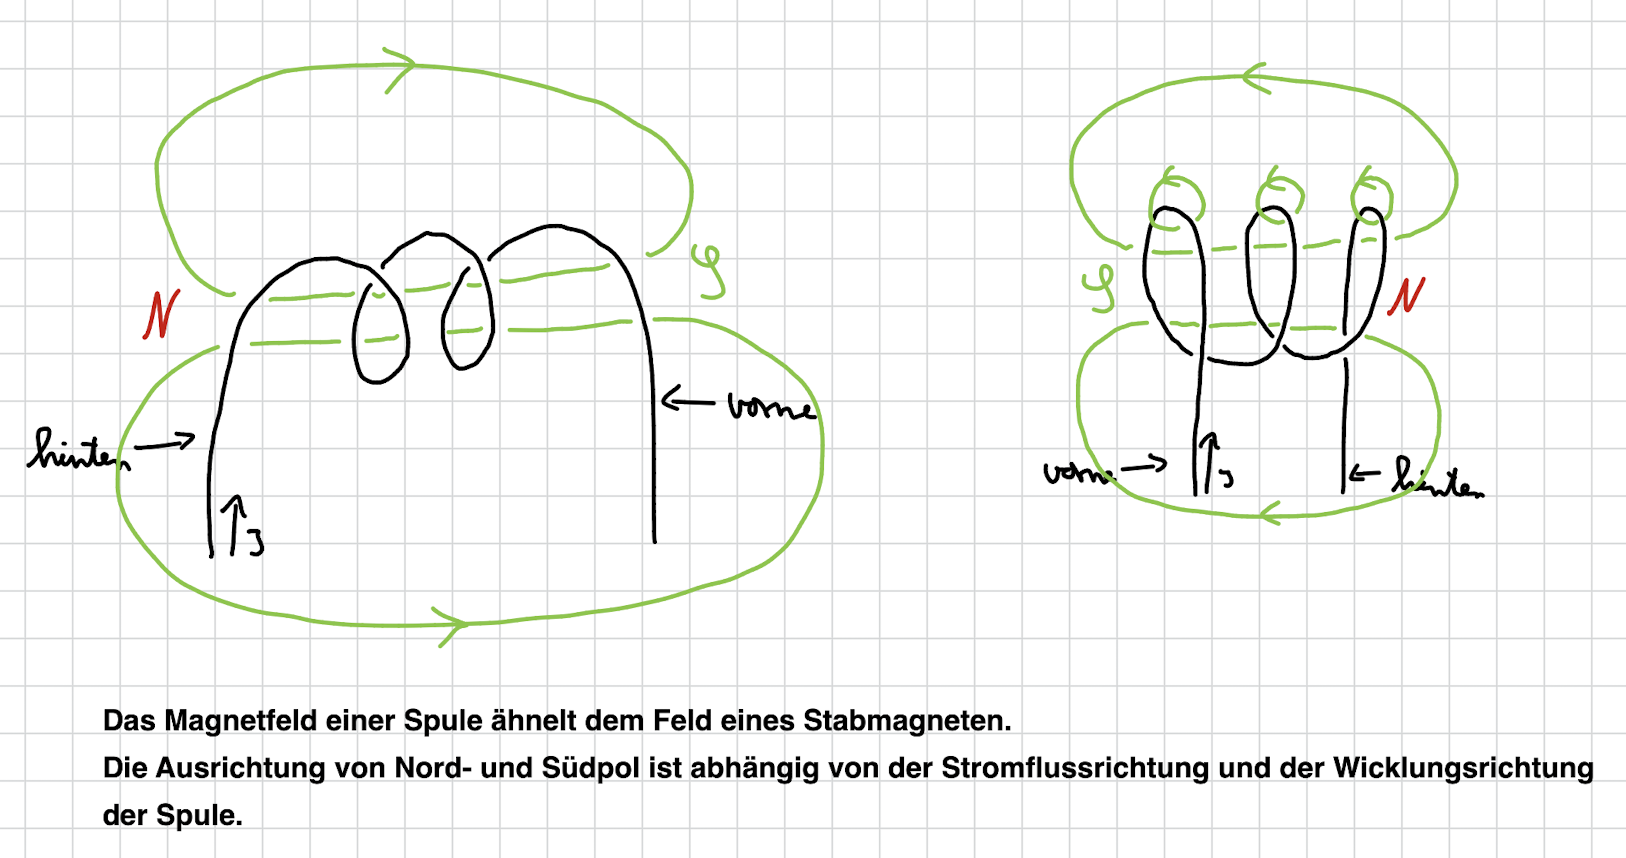
\includegraphics[width=\textwidth]{Images/Das Magnetfeld einer stromdurchflossenen Spule.png}
	\newpage
	\section{Die Stromwaage}
	\vspace{0.5cm}
	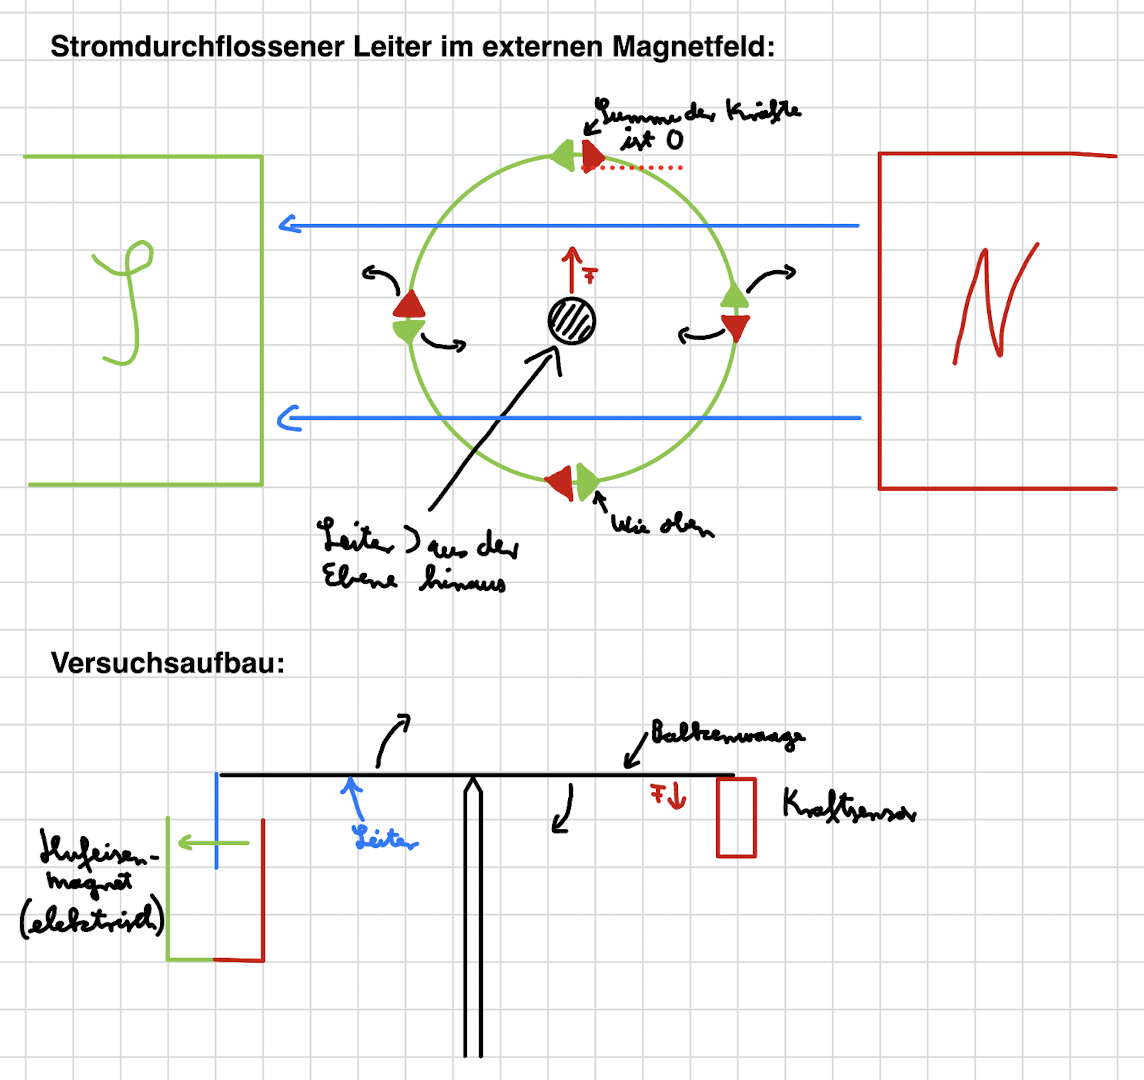
\includegraphics[height=0.5\textwidth]{Images/Die Stromwaage.png}
	\hfill
	\includegraphics[height=0.5\textwidth]{Images/Durchführung - Die Stromwaage.png}\\
	\vspace{0.5cm}
	
	\begin{enumerate}[itemsep=0pt]
		\item Werte in Tabelle in TR eingetragen
		\item Diagramm anlegen:
		\begin{itemize} [topsep=-4pt, itemsep=-4pt]
			\item x-Achse: F in mN
			\item y-Achse: I in A
		\end{itemize}
		\item Die Punkte verlaufen augenscheinlich entlang einer Geraden\\
		$\rightarrow$ Lineare Regression: $6.55x-0.8$
		\item Im physikalischen Zusammenhang: $6.55 \frac{mN}{A} \cdot I - 0.8 mN$ \qquad (für $F \sim l = 5.52 \frac{mN}{cm} \cdot l - 1.2\,\text{mN})$ \\
		$\rightarrow F(0) = -0.8$ wegen falscher Nullung des Kraftmessers.
	\end{enumerate}
	\begin{alignat}{3}
		&& \hspace{2cm} F(I) &= 0.0065 \frac{N}{A} \cdot I && \\[2pt]
		\Rightarrow && F &\sim I,\; F \sim l && \\
		\Rightarrow&& F &\sim I \cdot l && \\
		\Rightarrow && F &= k \cdot I \cdot l && \mid k = \text{B-Feld} \\
		\Rightarrow&& 0.0065 \frac{N}{A} &= k \cdot l && \\
		\Rightarrow && k = \frac{0.0065 \frac{N}{A}}{l} &= 0.131 \frac{N}{A\,m} && \\[6pt]
		&& 0.552 \frac{N}{m} &= k \cdot I && \\
		&& k &= \frac{0.552 \frac{N}{m}}{4A} = 0.138 \frac{N}{A\,m} && \\[10pt]
		&& \frac{N}{A\,m} = \frac{kg\,\frac{m}{s^2}}{A\,m} &= \frac{kg}{A\,s^2} = \text{Tesla} = T &&
	\end{alignat}
	\newpage
	
	\section{Die magnetische Flussdichte ("Magnetfeld")}
	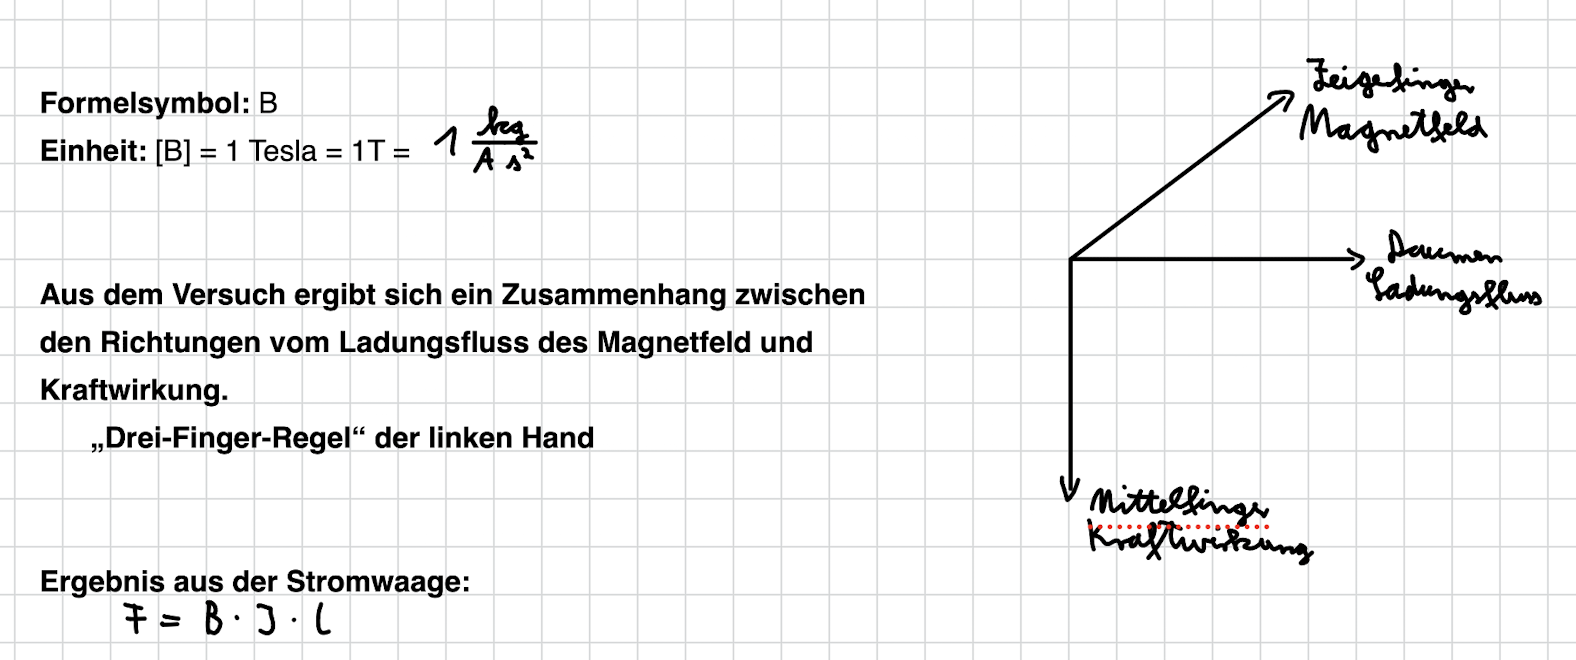
\includegraphics[width=\textwidth]{Images/Die magnetische Flussdichte.png}
	\newpage
	
	
	
	\section{Die Lorentzkraft}
	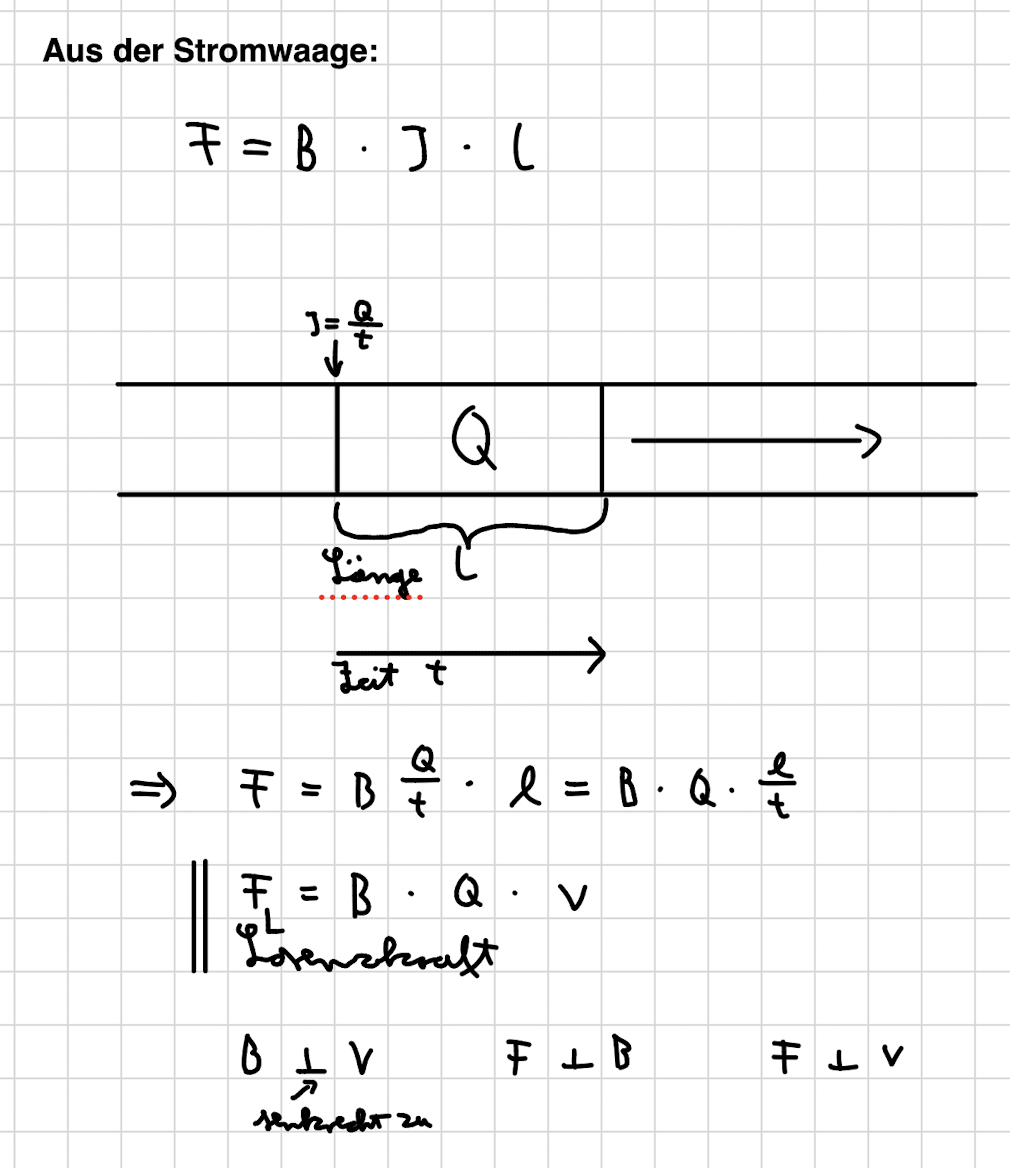
\includegraphics[width=0.6\textwidth]{Images/Die Lorentzkraft.png}
	\subsection{Hausaufgabe}
	\begin{alignat}{2}
		\dkreis{1} \hspace{2cm}
		1.9\cdot10^{11} \frac{C}{kg} \cdot e^- &= m_e \qquad \mid KW\\
		\frac{1}{1.9\cdot 10^{11}} \frac{kg}{C} \cdot e^- &= m_e\\
		\Rightarrow m_e &= 8.43 \cdot 10^{-31} kg \qquad\\
		(\text{Literaturwert} \quad m_e &= 9.11 \cdot 10^{-31} kg)
	\end{alignat}
	\begin{minipage}[H]{0.7\textwidth}
		\begin{alignat}{2}
			\dkreis{2} \hspace{2cm}
			U_B = ? \qquad r &= 10cm \qquad B = 2mT &\\
			\frac{e^-}{m_e} &= \frac{2 U_B}{r^2 B^2} & \mid \cdot r^2 \cdot B^2\\
			\frac{e^- \cdot r^2 \cdot B^2}{m_e} &= 2U_B &\mid :2\\
			U_B &= \frac{e^-}{m_e} \frac{r^2 B^2}{2} &\\
			&= 1.7588 \cdot 10^{11} \frac{C}{kg} \cdot \frac{(0.1m)^2 \cdot (0.002T)^2}{2}\\
			&= 3517.6 V
		\end{alignat}
	\end{minipage}
	\hfill
	\begin{minipage}[H]{0.2\textwidth}
		\begin{tcolorbox}[colframe=black, colback=white, left=0pt, right=0pt, boxsep=0pt]
			\begin{alignat}{1}
				&\frac{C}{kg} \cdot m^2 \cdot T^2\\
				=& \frac{C}{kg} m^2 \left(\frac{kg}{Cs}\right)^2 \\
				=& \frac{kg \cdot m^2}{Cs^2}\\
				=& \frac{J}{C}\\
				=& \frac{CV}{C} \\
				=& V
			\end{alignat}
		\end{tcolorbox}
	\end{minipage}
	
	\newpage
	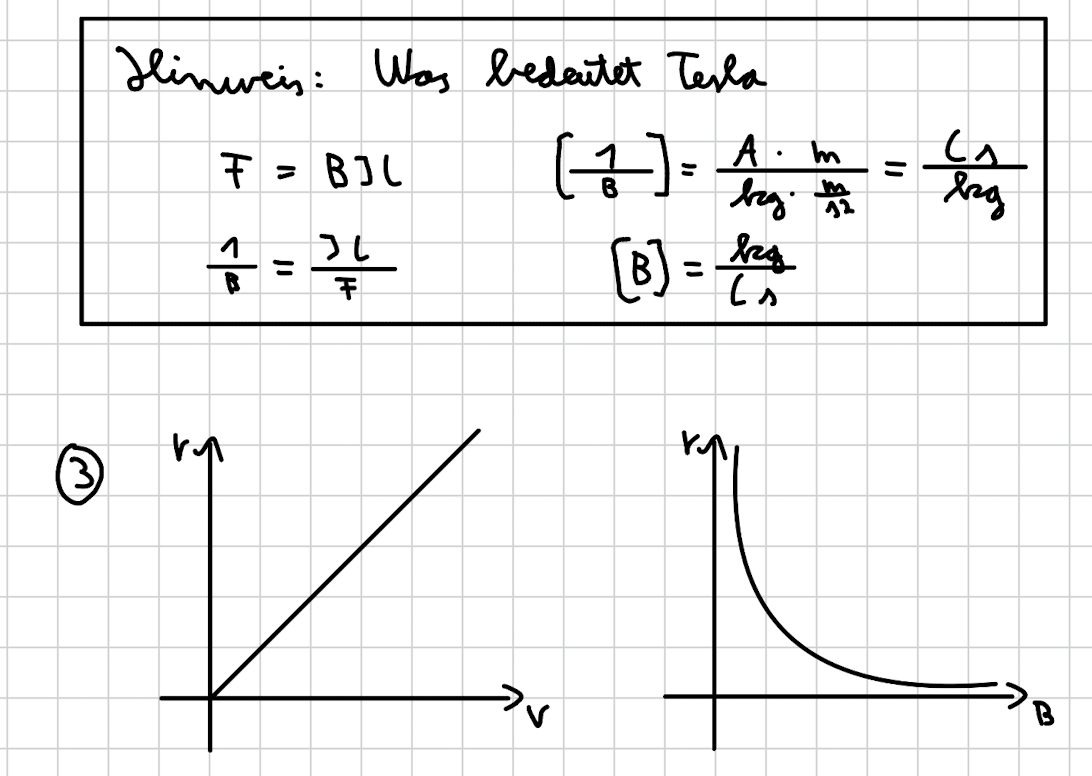
\includegraphics[width=0.7\textwidth]{Images/Was bedeutet Tesla.png}

	
	\newpage
	\section{Das Fadenstrahlrohr}
	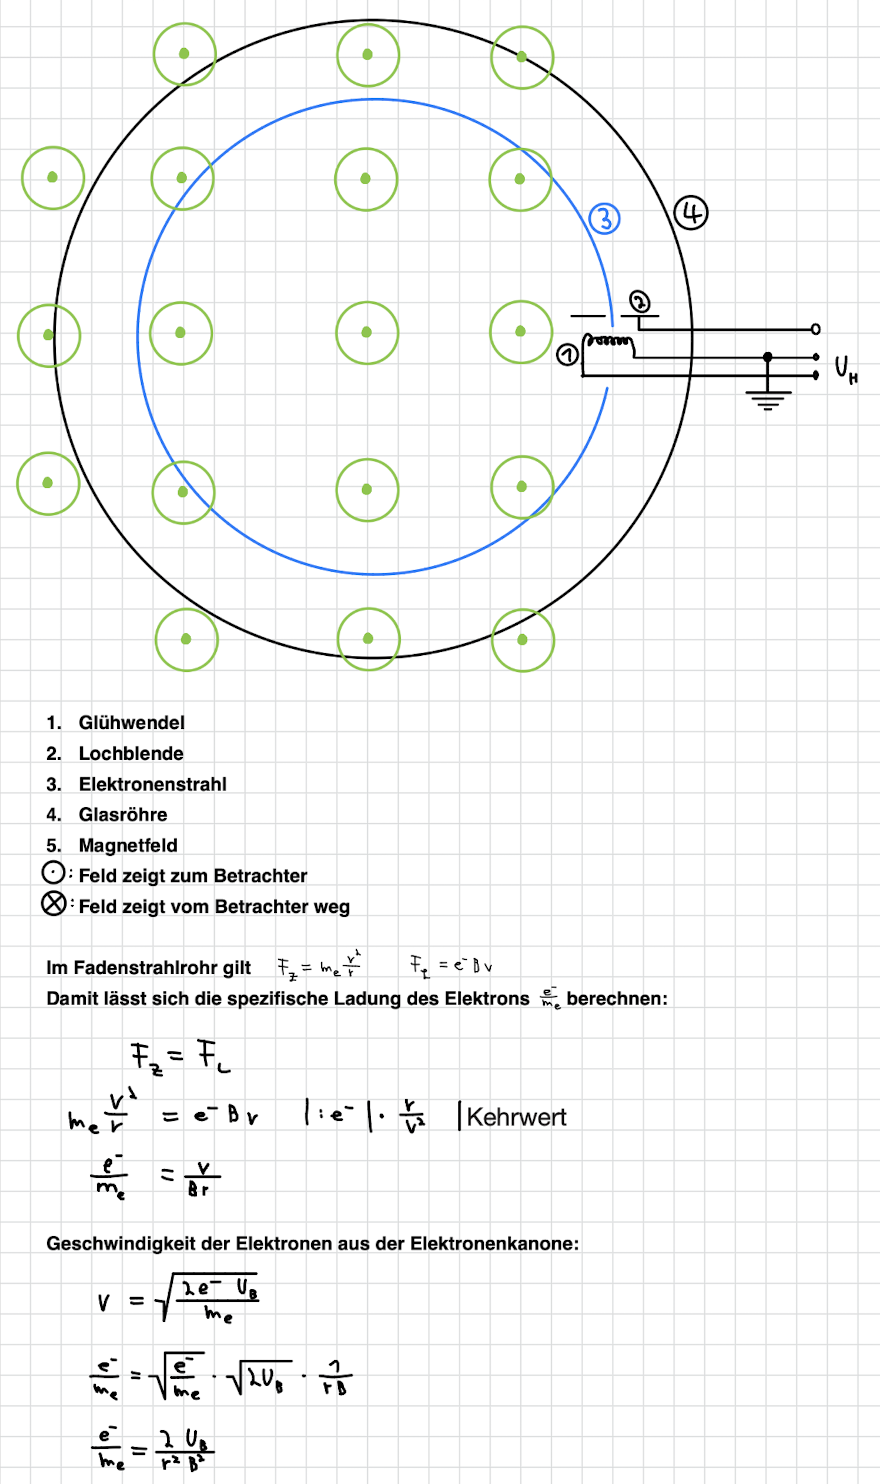
\includegraphics[height=\textheight]{Images/Das Fadenstrahlrohr.png}
	\newpage
	
	\section{Magnetfeld einer Helmholtzspule}
	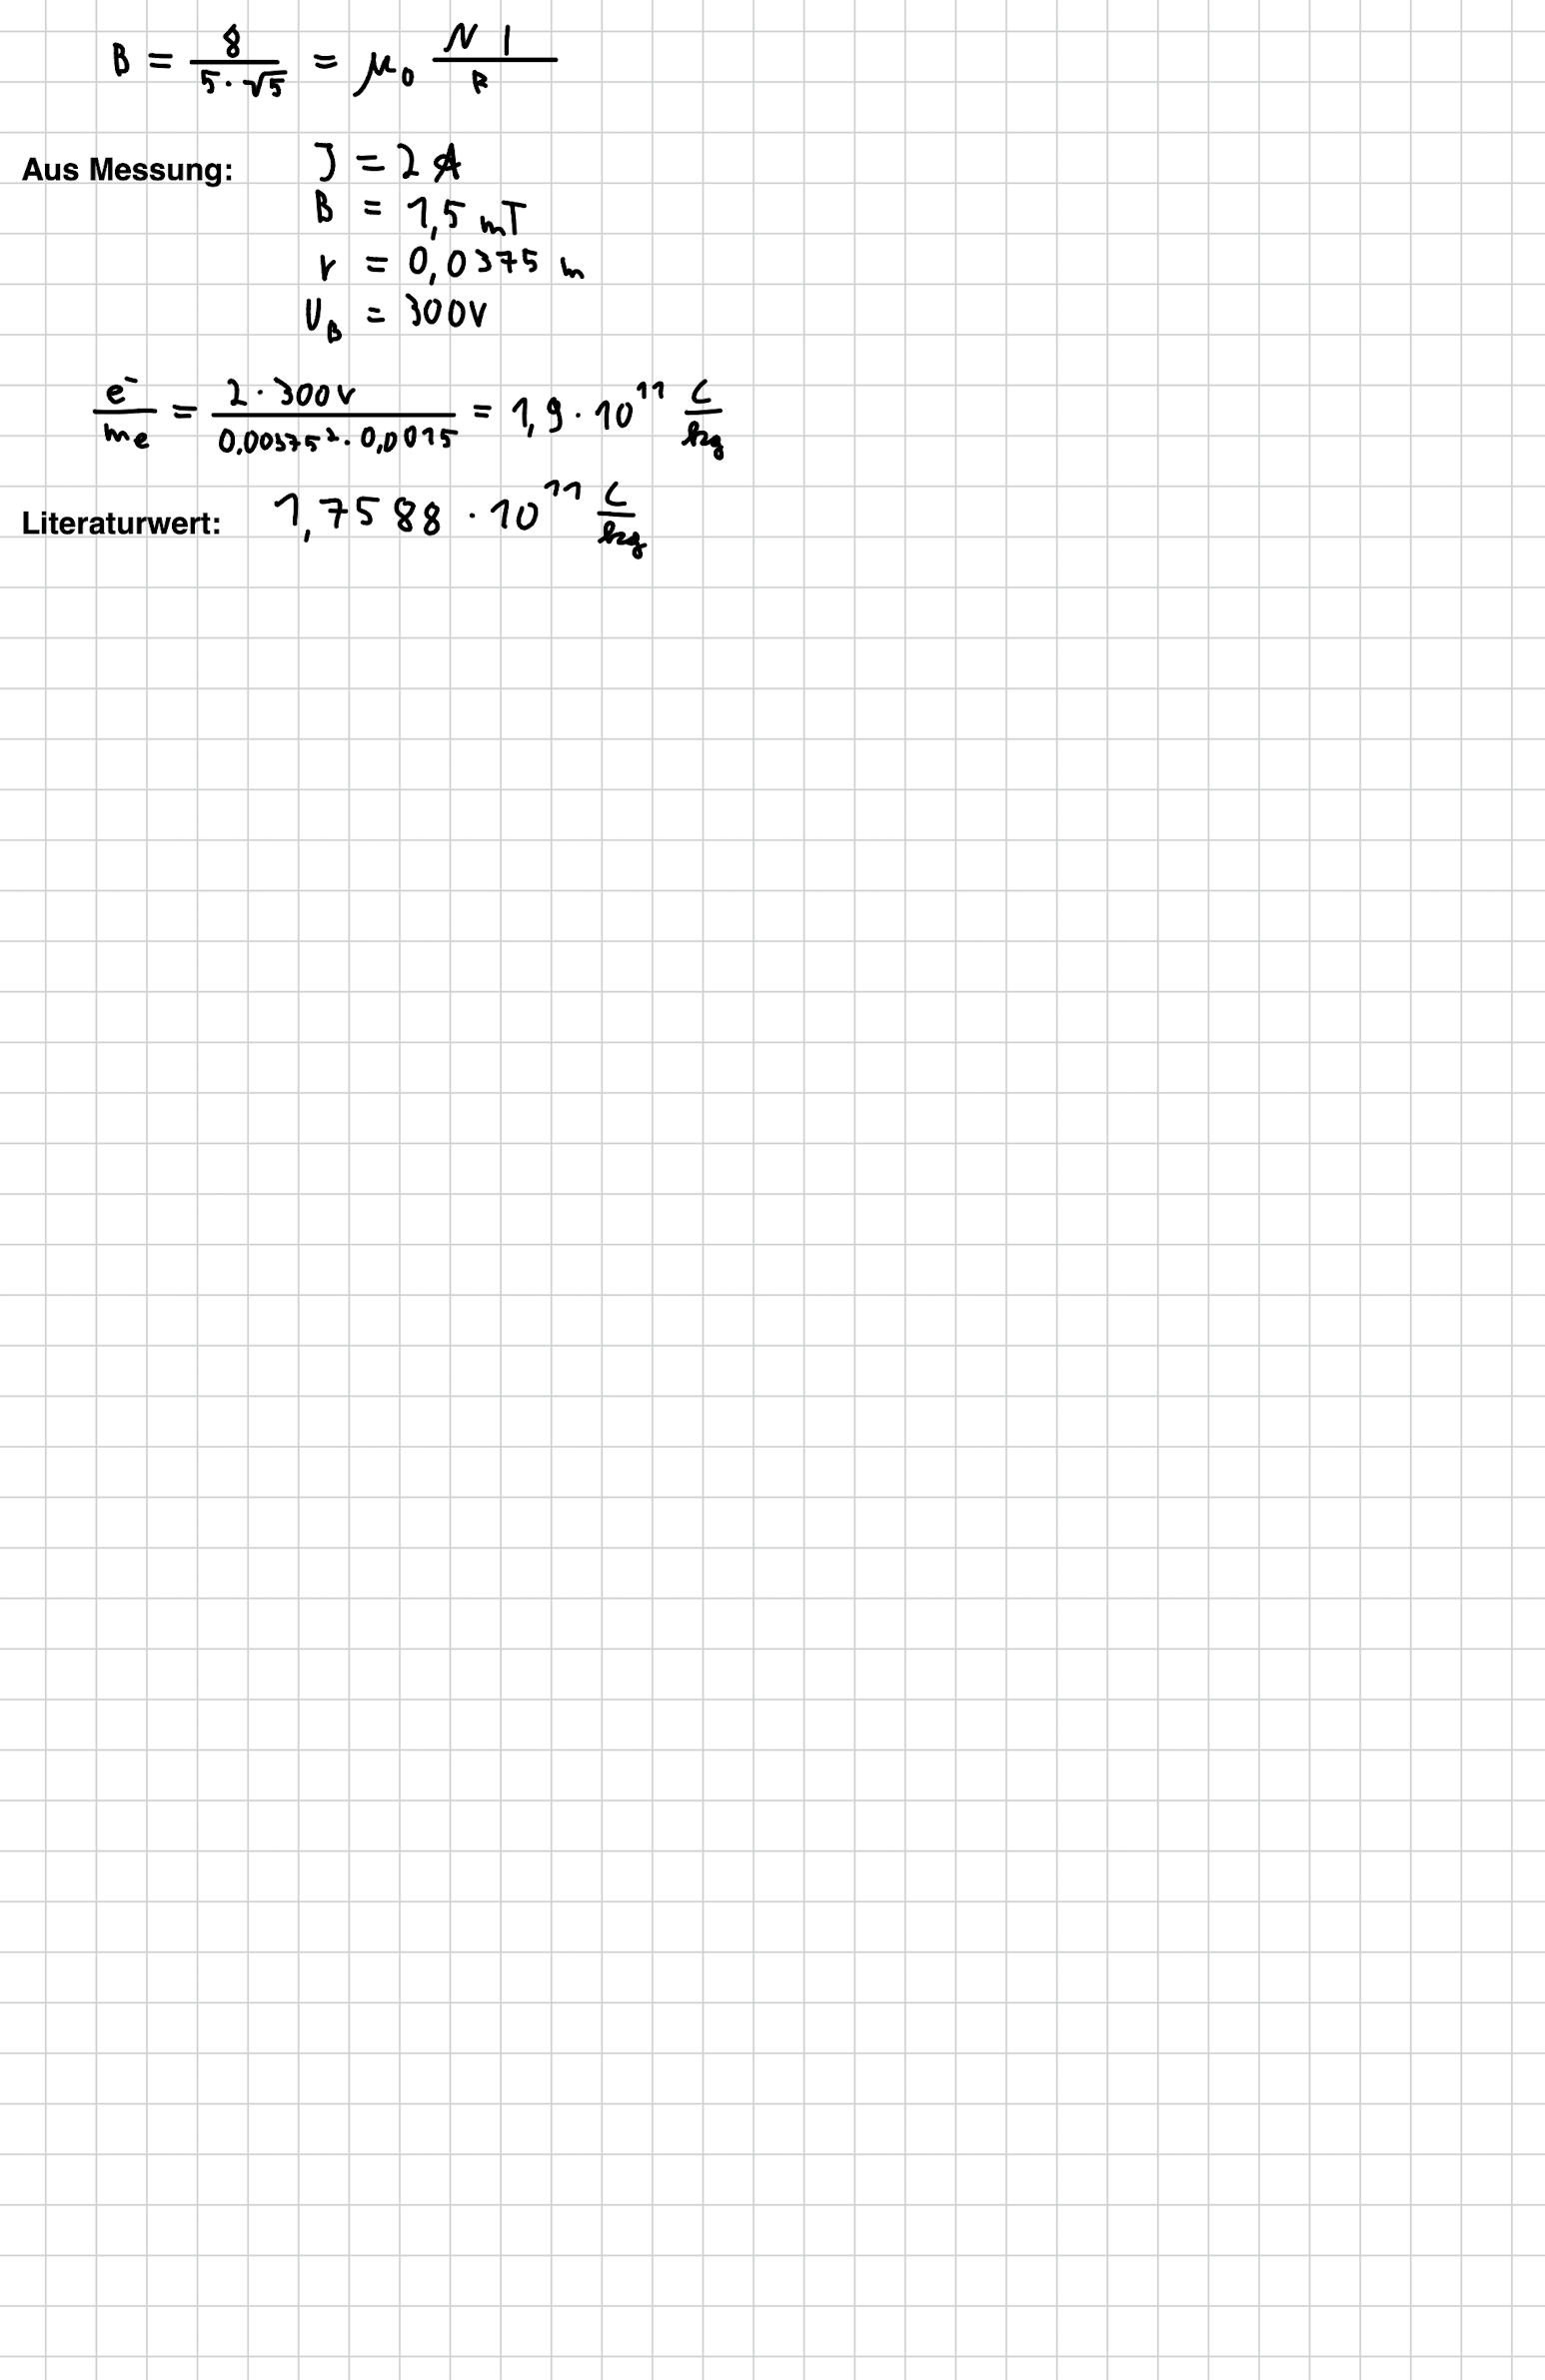
\includegraphics[height=\textheight]{Images/Helmkoltzspule.png}
	\newpage
	\section{Der Wienfilter}
	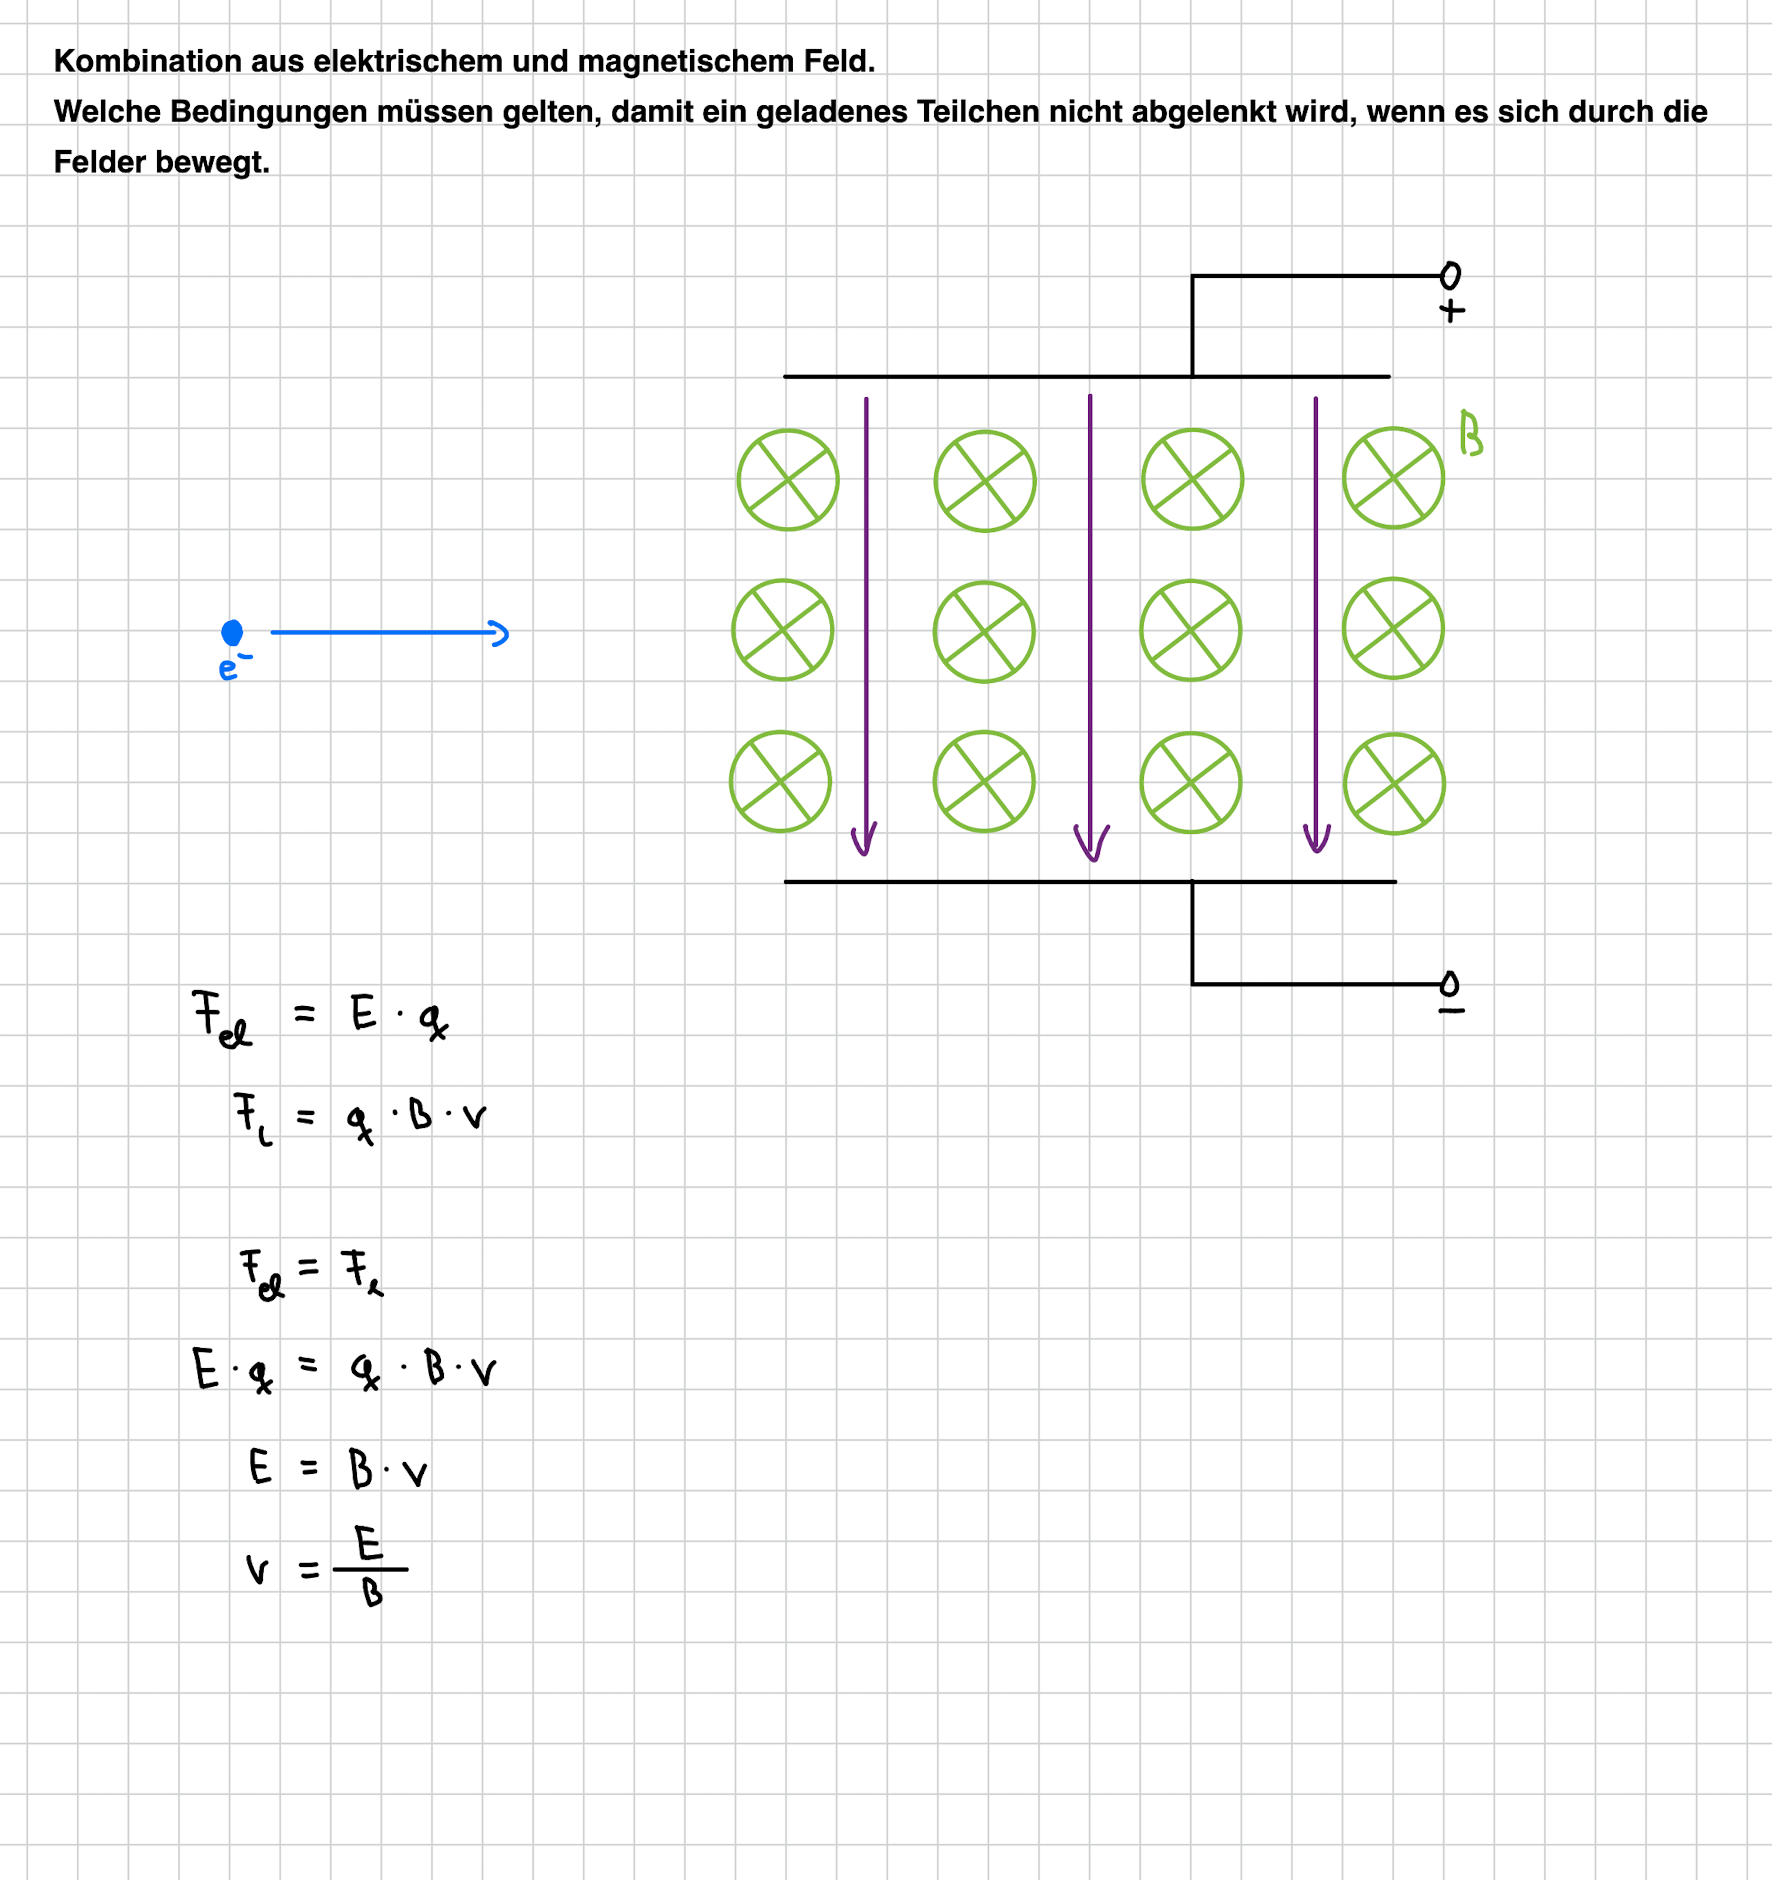
\includegraphics[width=\textwidth]{Images/Wienfilter.png}
	\newpage
	\section{Das Massenspektrometer}
	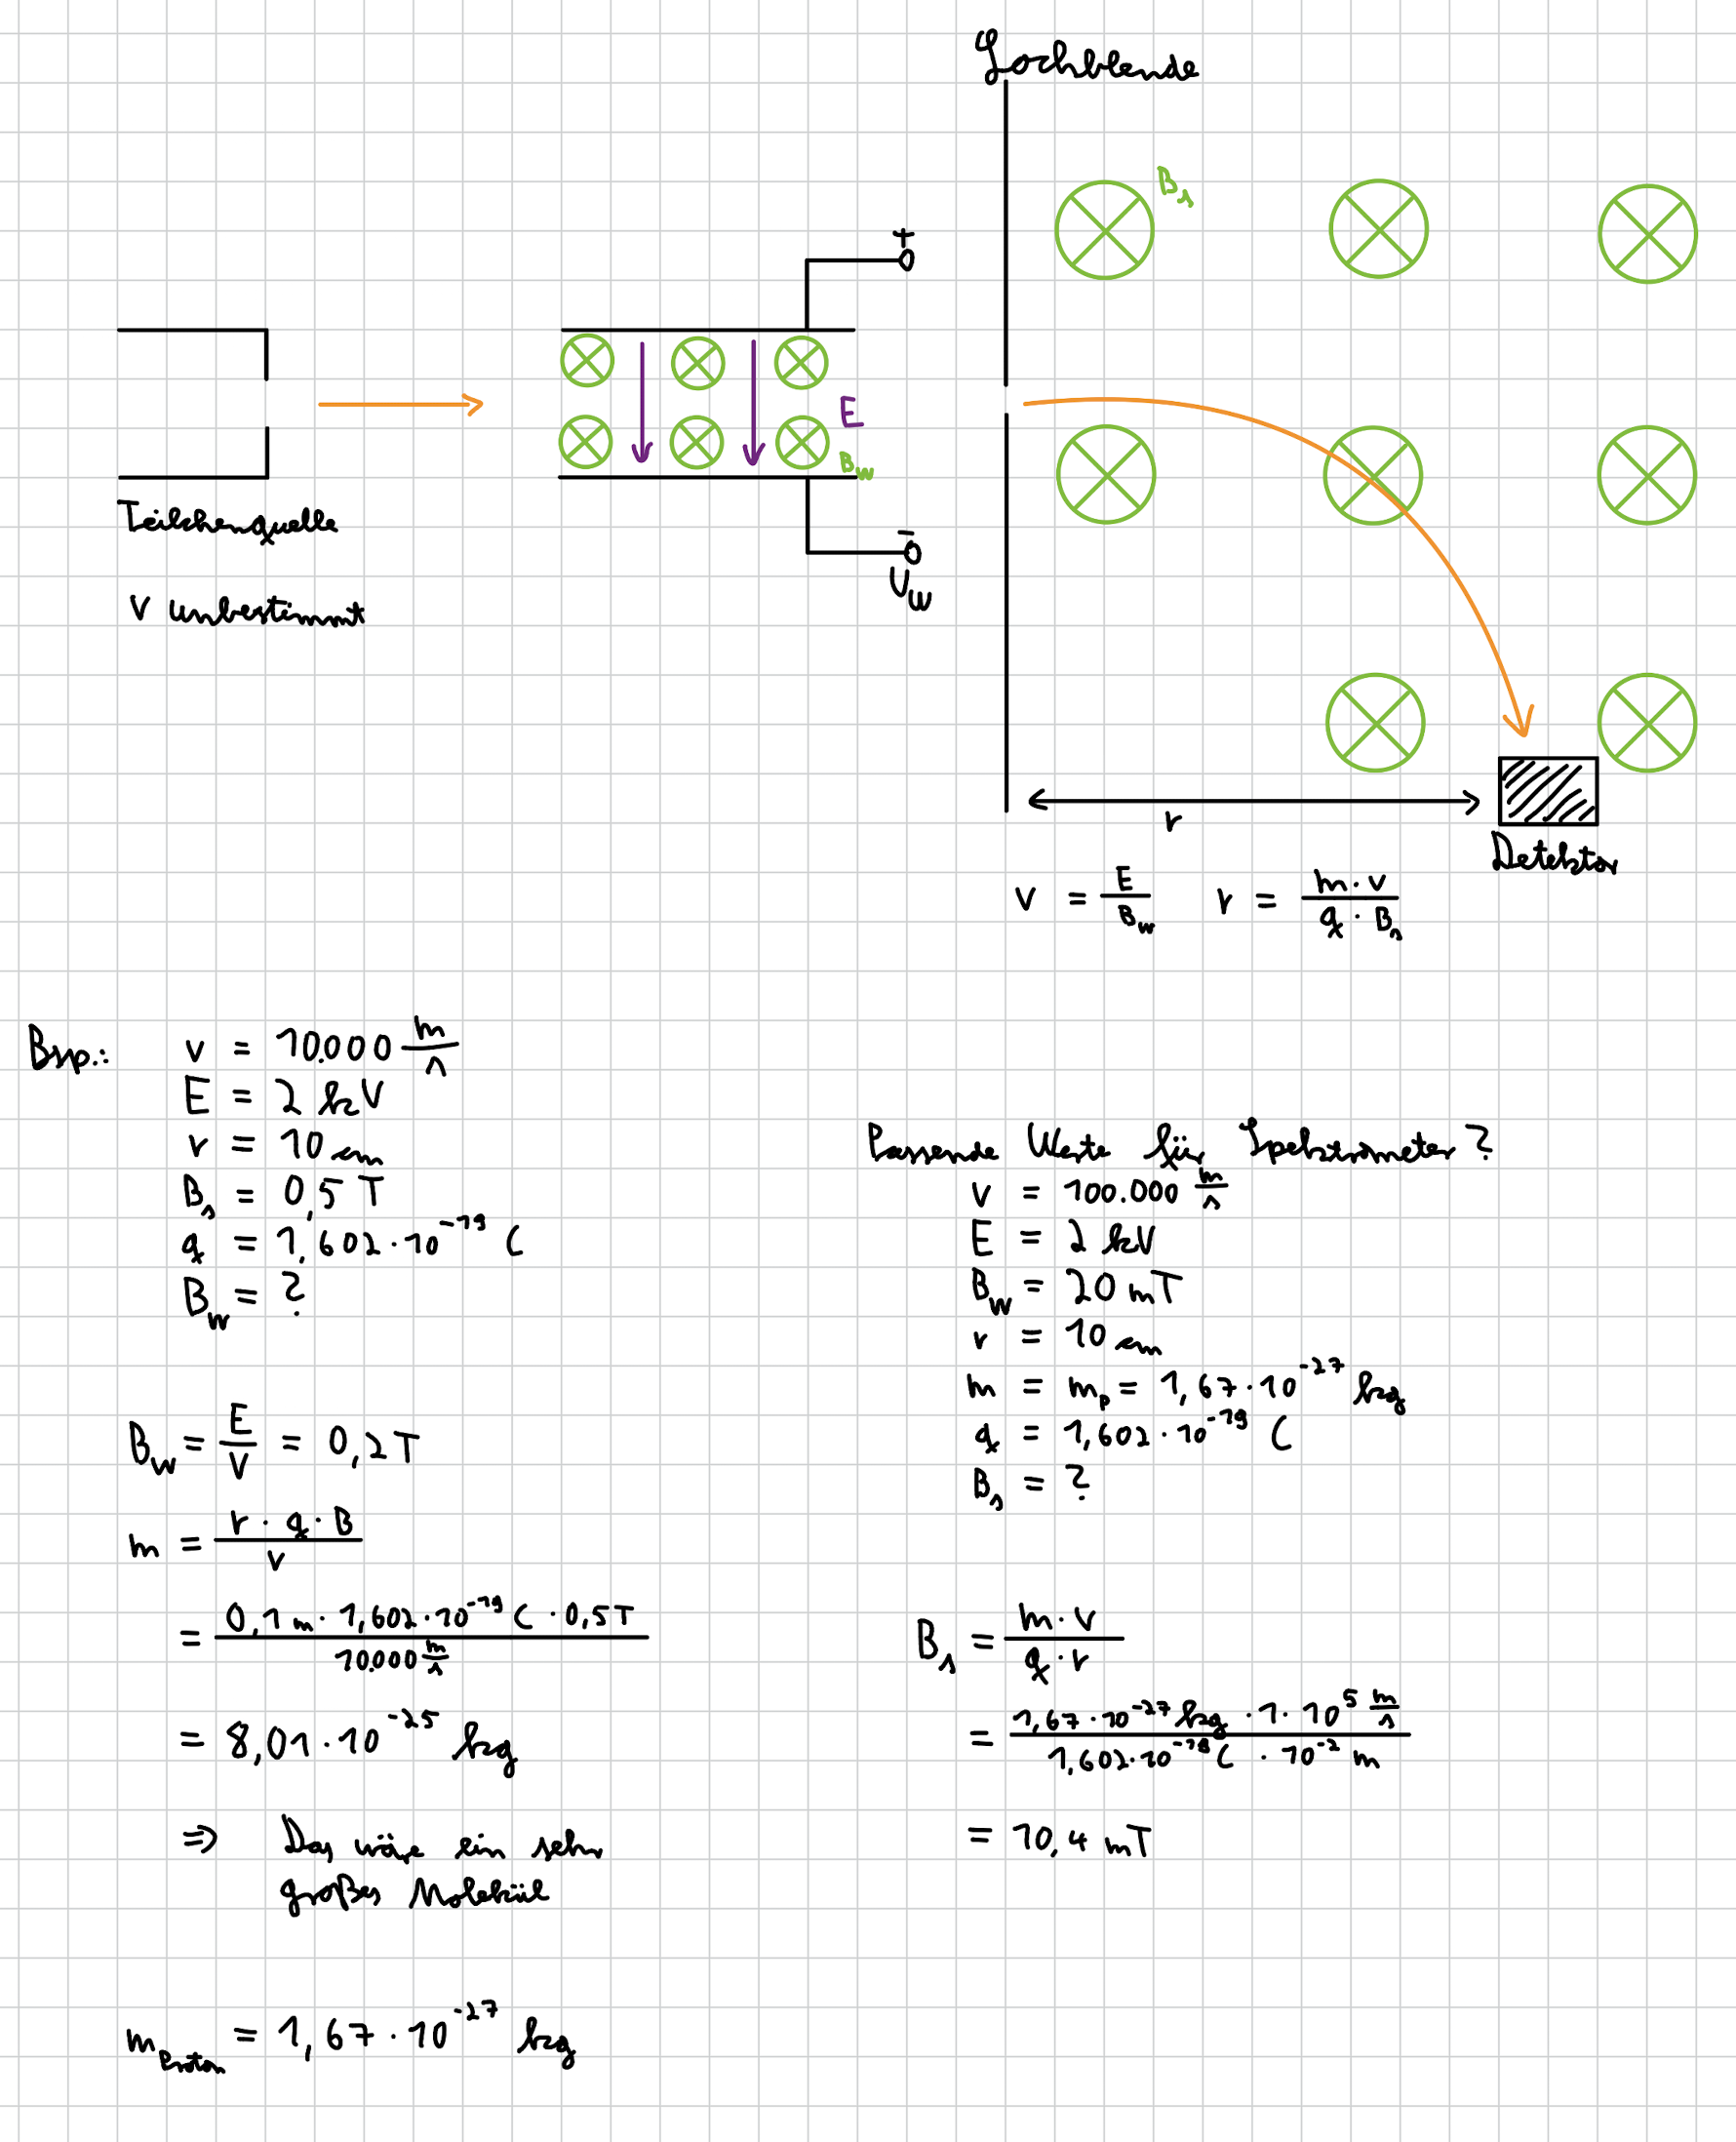
\includegraphics[width=\textwidth]{Images/Massenspektrometer.png}
	\newpage
	\section{Der Hall-Effekt}
	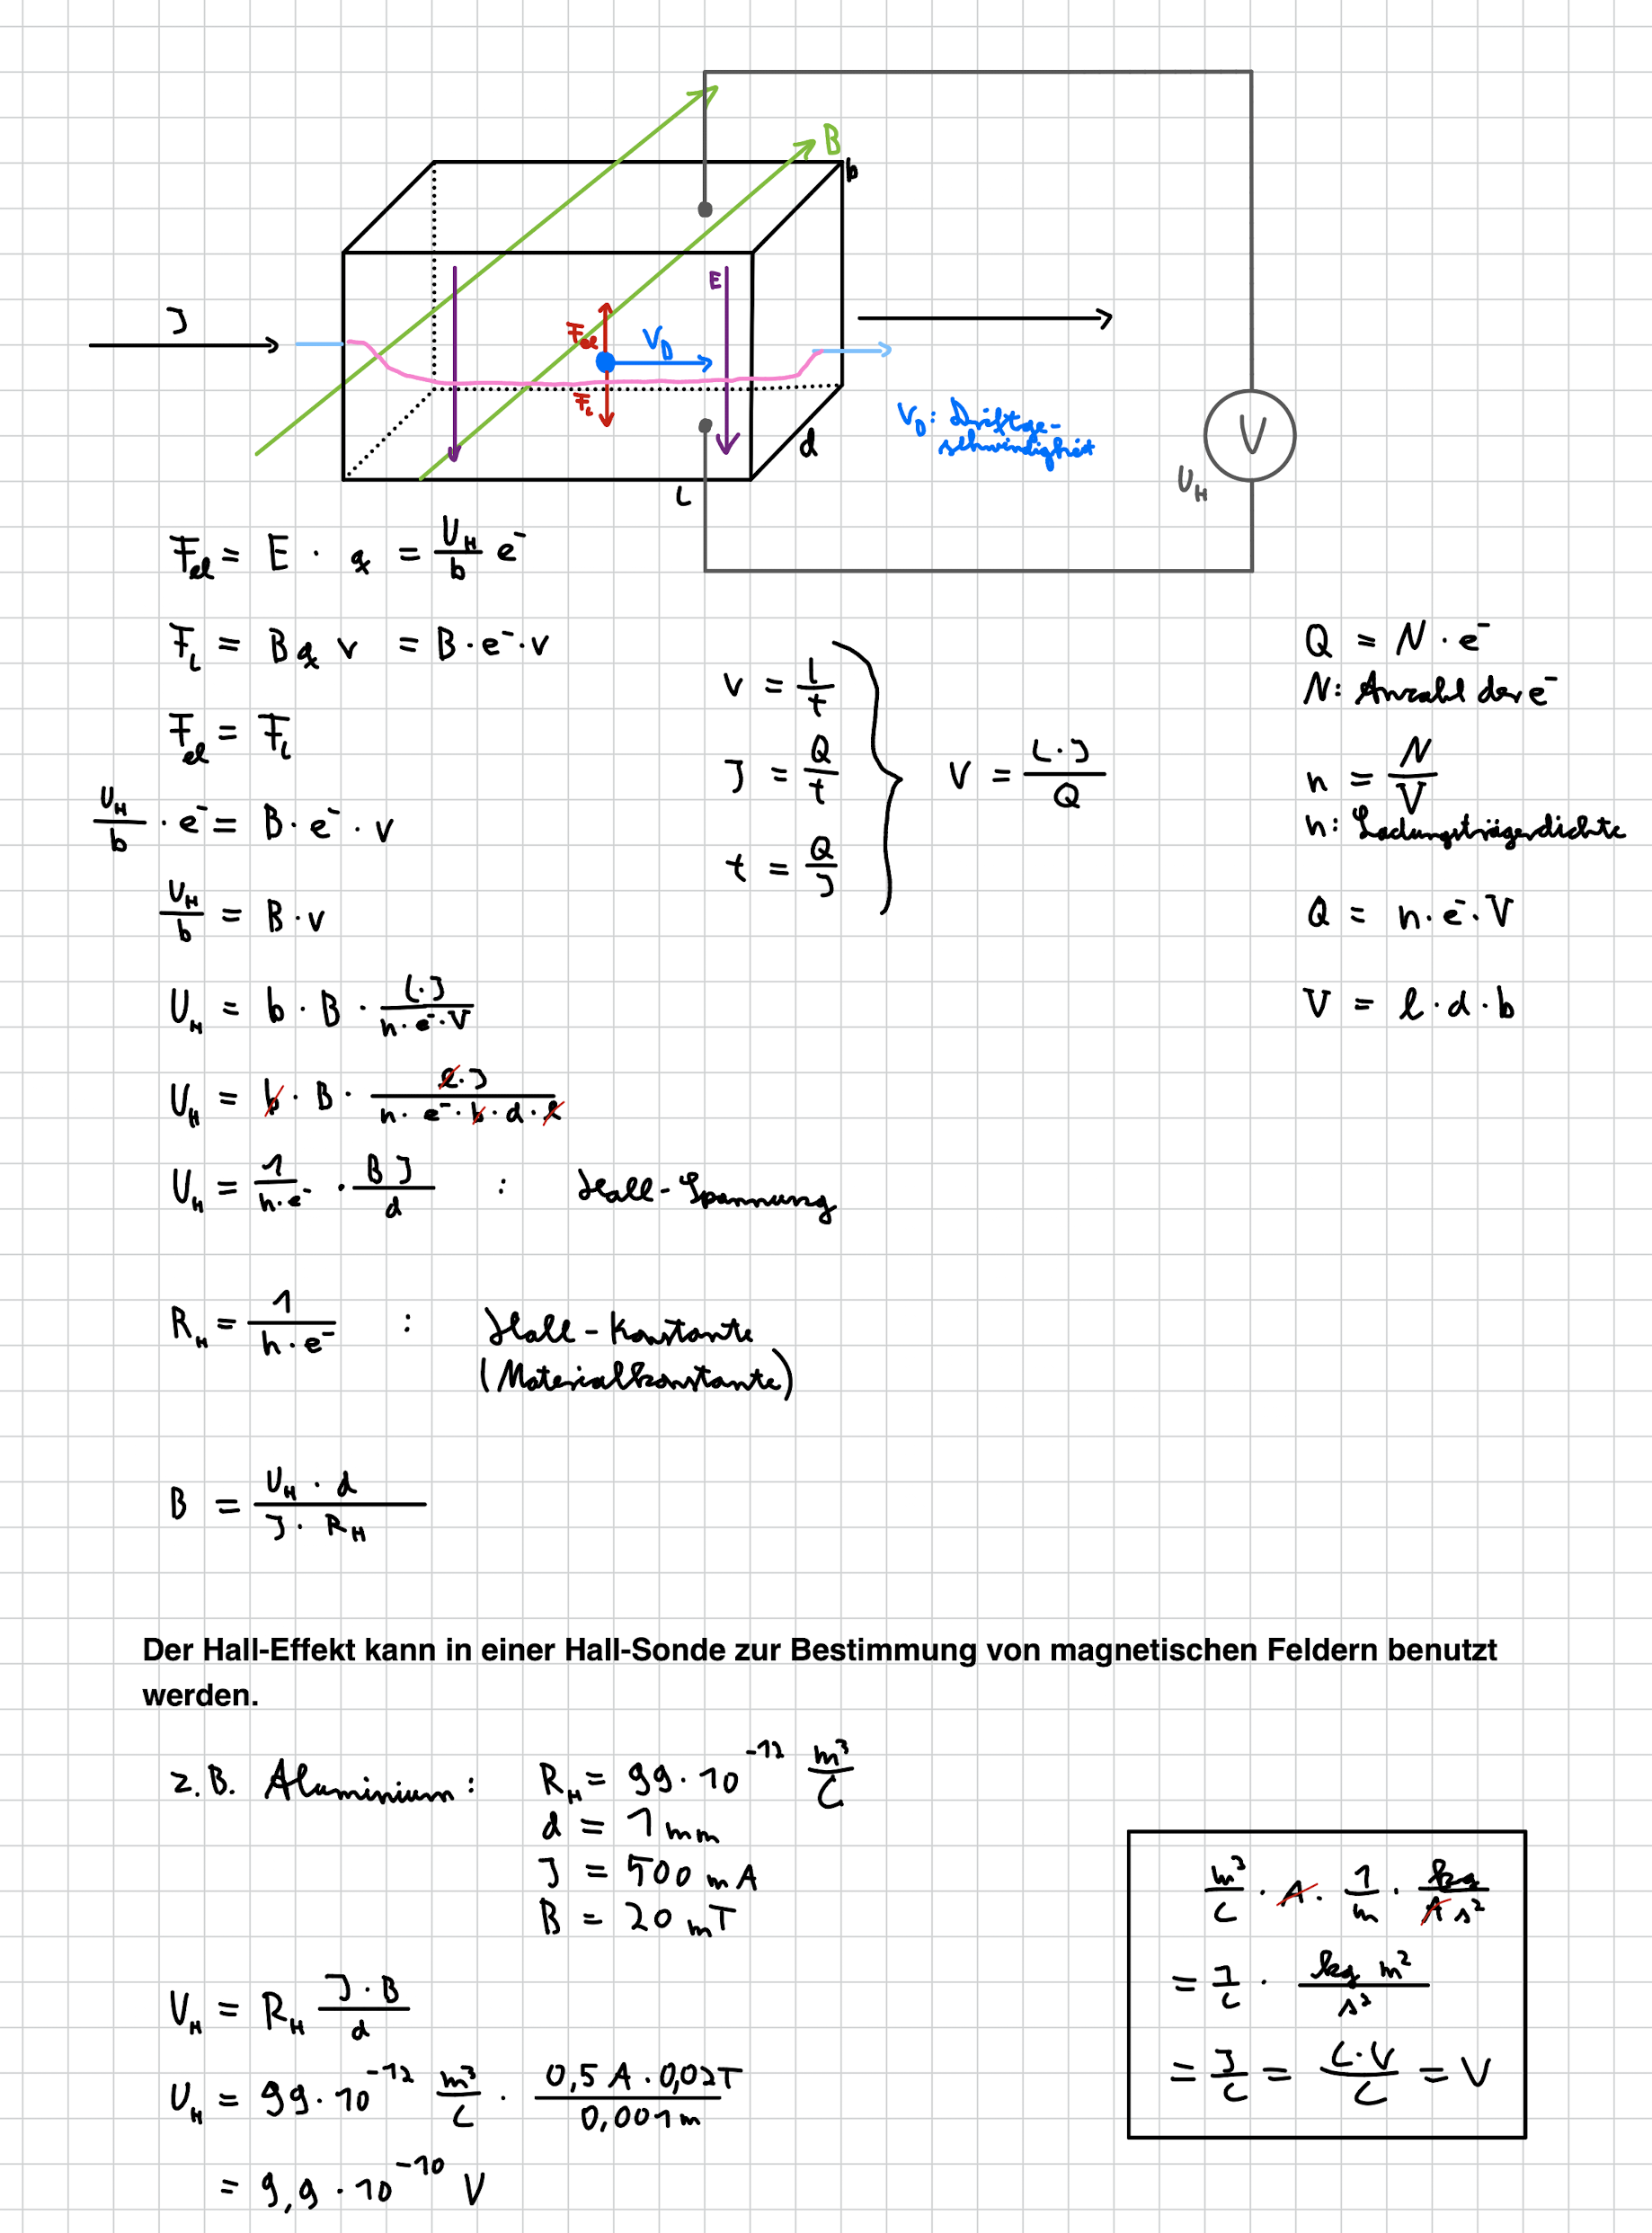
\includegraphics[width=0.9\textwidth]{Images/Hall-Effekt.png}
	\newpage
	\section{Magnetfeld einer Spule - quantitativ}
	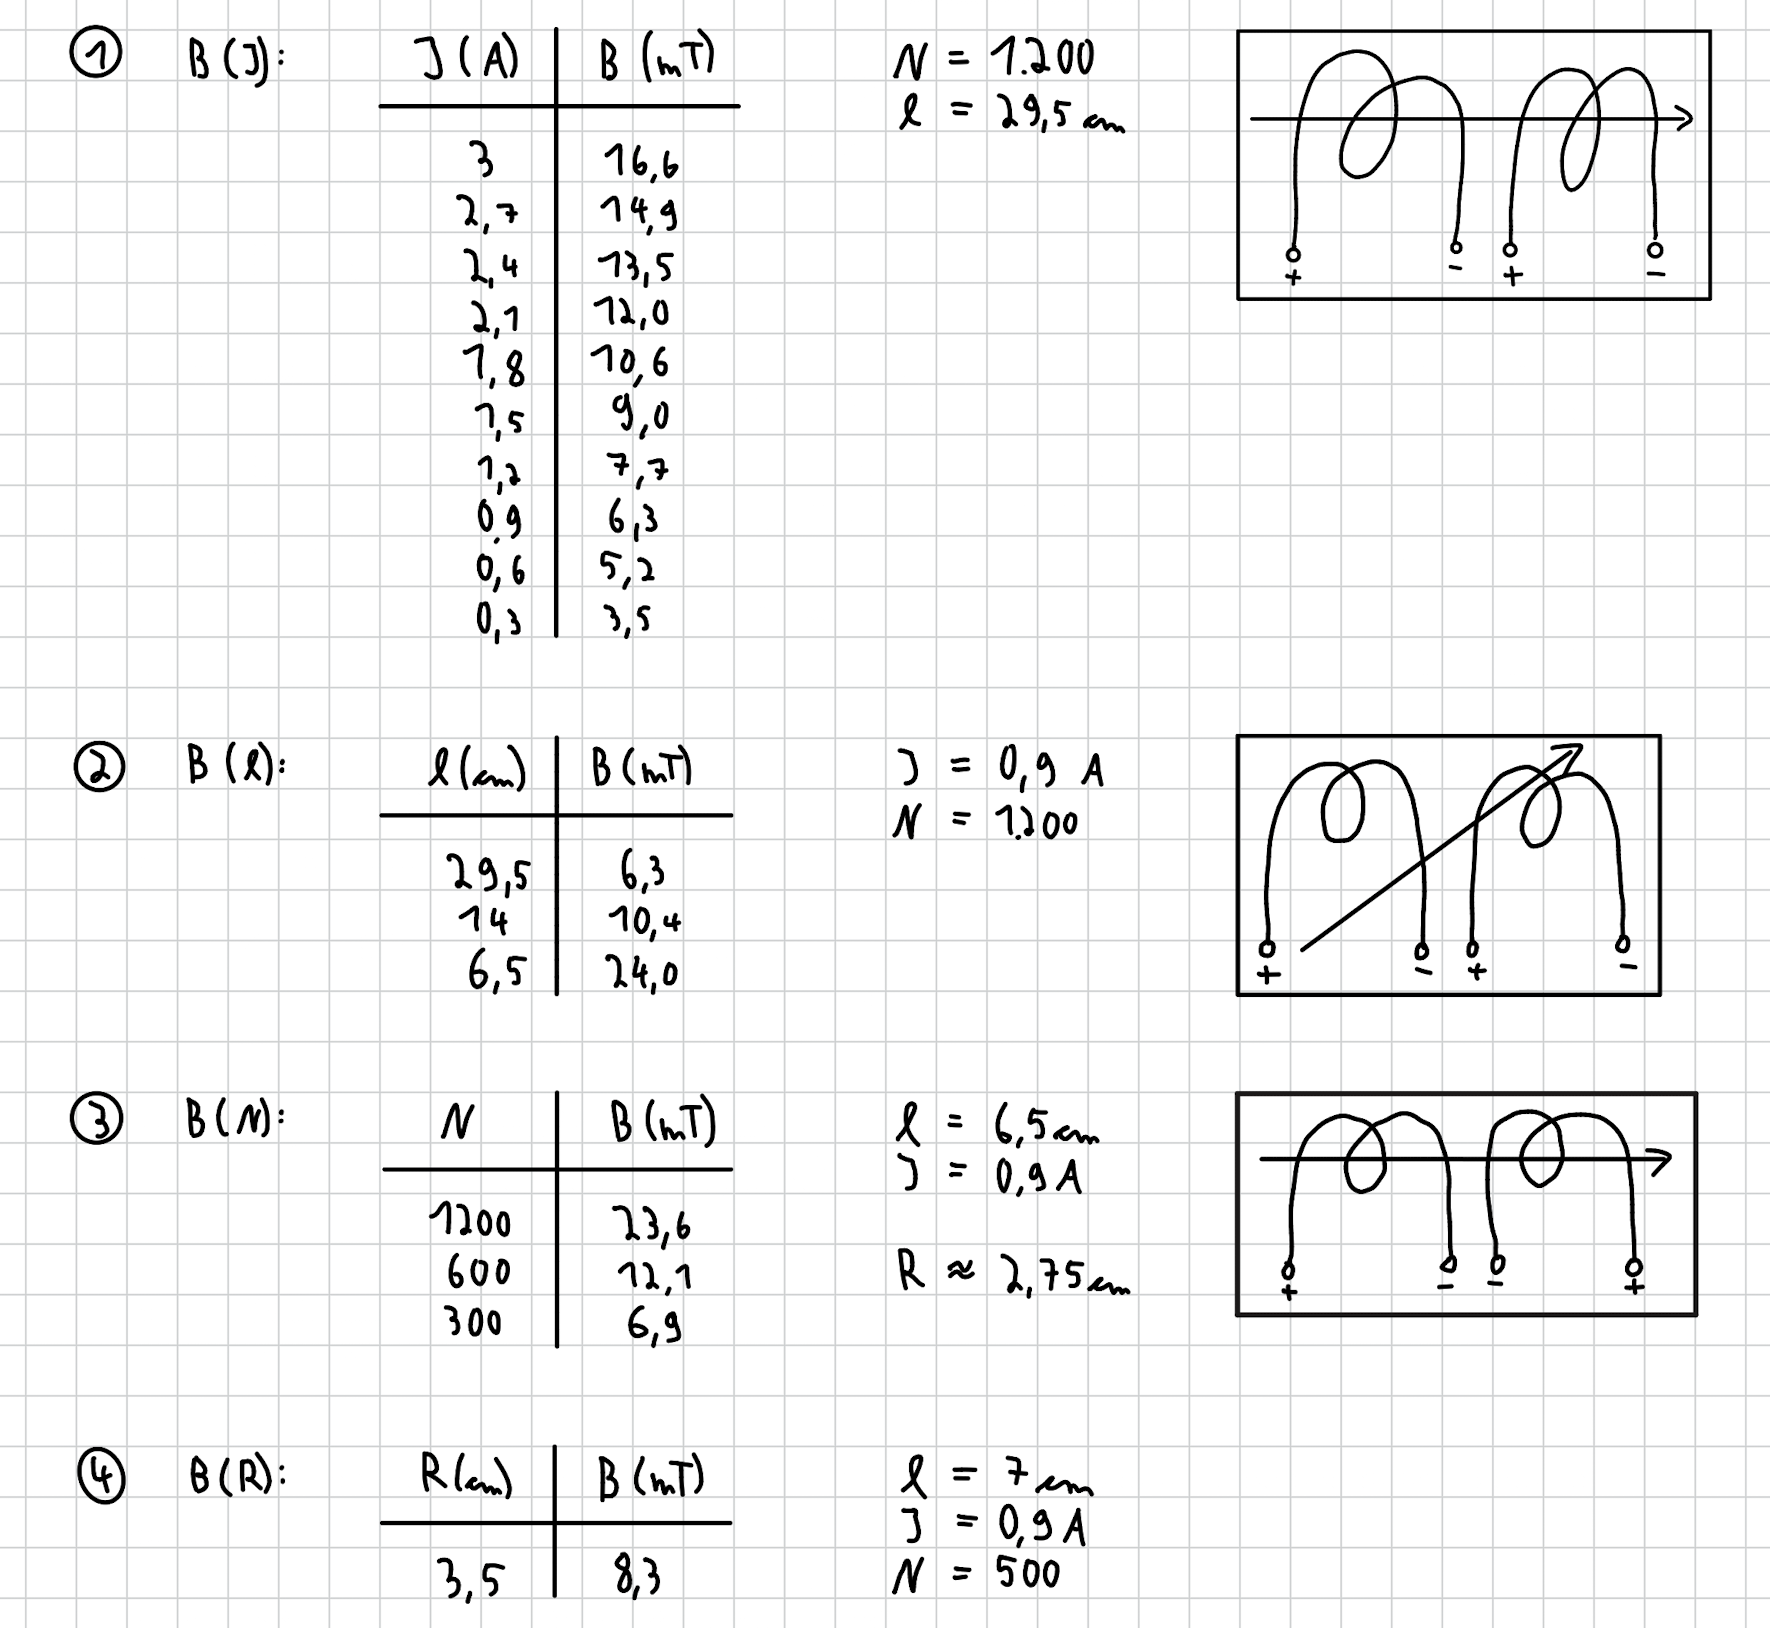
\includegraphics[width=\textwidth]{Images/Magnetfeld einer Spule quantitativ.png}
	\\


	\begin{minipage}[t]{0.48\textwidth}
		\textbf{Aus B(N)}
		\begin{alignat}{1}
			0.0186 mT &= k \cdot I \cdot \frac{1}{r}\\
			k &= \frac{0.0186 mT \cdot 0.06 m}{0.9 A}\\
			&= 1.326 \cdot 10^{-6} \frac{N}{A^2} \\
		\end{alignat}
	\end{minipage}
	\hfill
	\begin{minipage}[t]{0.48\textwidth}
		\textbf{Aus B(I):}
		\begin{alignat}{1}
			4.76364 \frac{mT}{A} &= k \cdot \frac{N}{C} \\
			k &= \frac{4.76364 \frac{mT}{A} \cdot 0.295 m}{1200}\\
			&= 1.171 \cdot 10^{-6} \frac{N}{A^2}\\
		\end{alignat}
	\end{minipage}
	


	\textbf{Mittelwert:} $\bar{k} = 1.46 \cdot 10^{-6} \frac{N}{A^2}$
	
	\vspace{0.5cm}
	\noindent
	Man nennt den Wert k magnetische Permeabilität des Vakuums oder magnetische Feldkonstante $\mu_0$\\
	Literaturwert: $1.256 \cdot 10^{-6} \frac{N}{A^2}$\\
	Es gilt: $\mu_0 = \frac{1}{\epsilon_0 c^2}$


	\newpage
	\section{Das Magnetfeld einer Spule}
	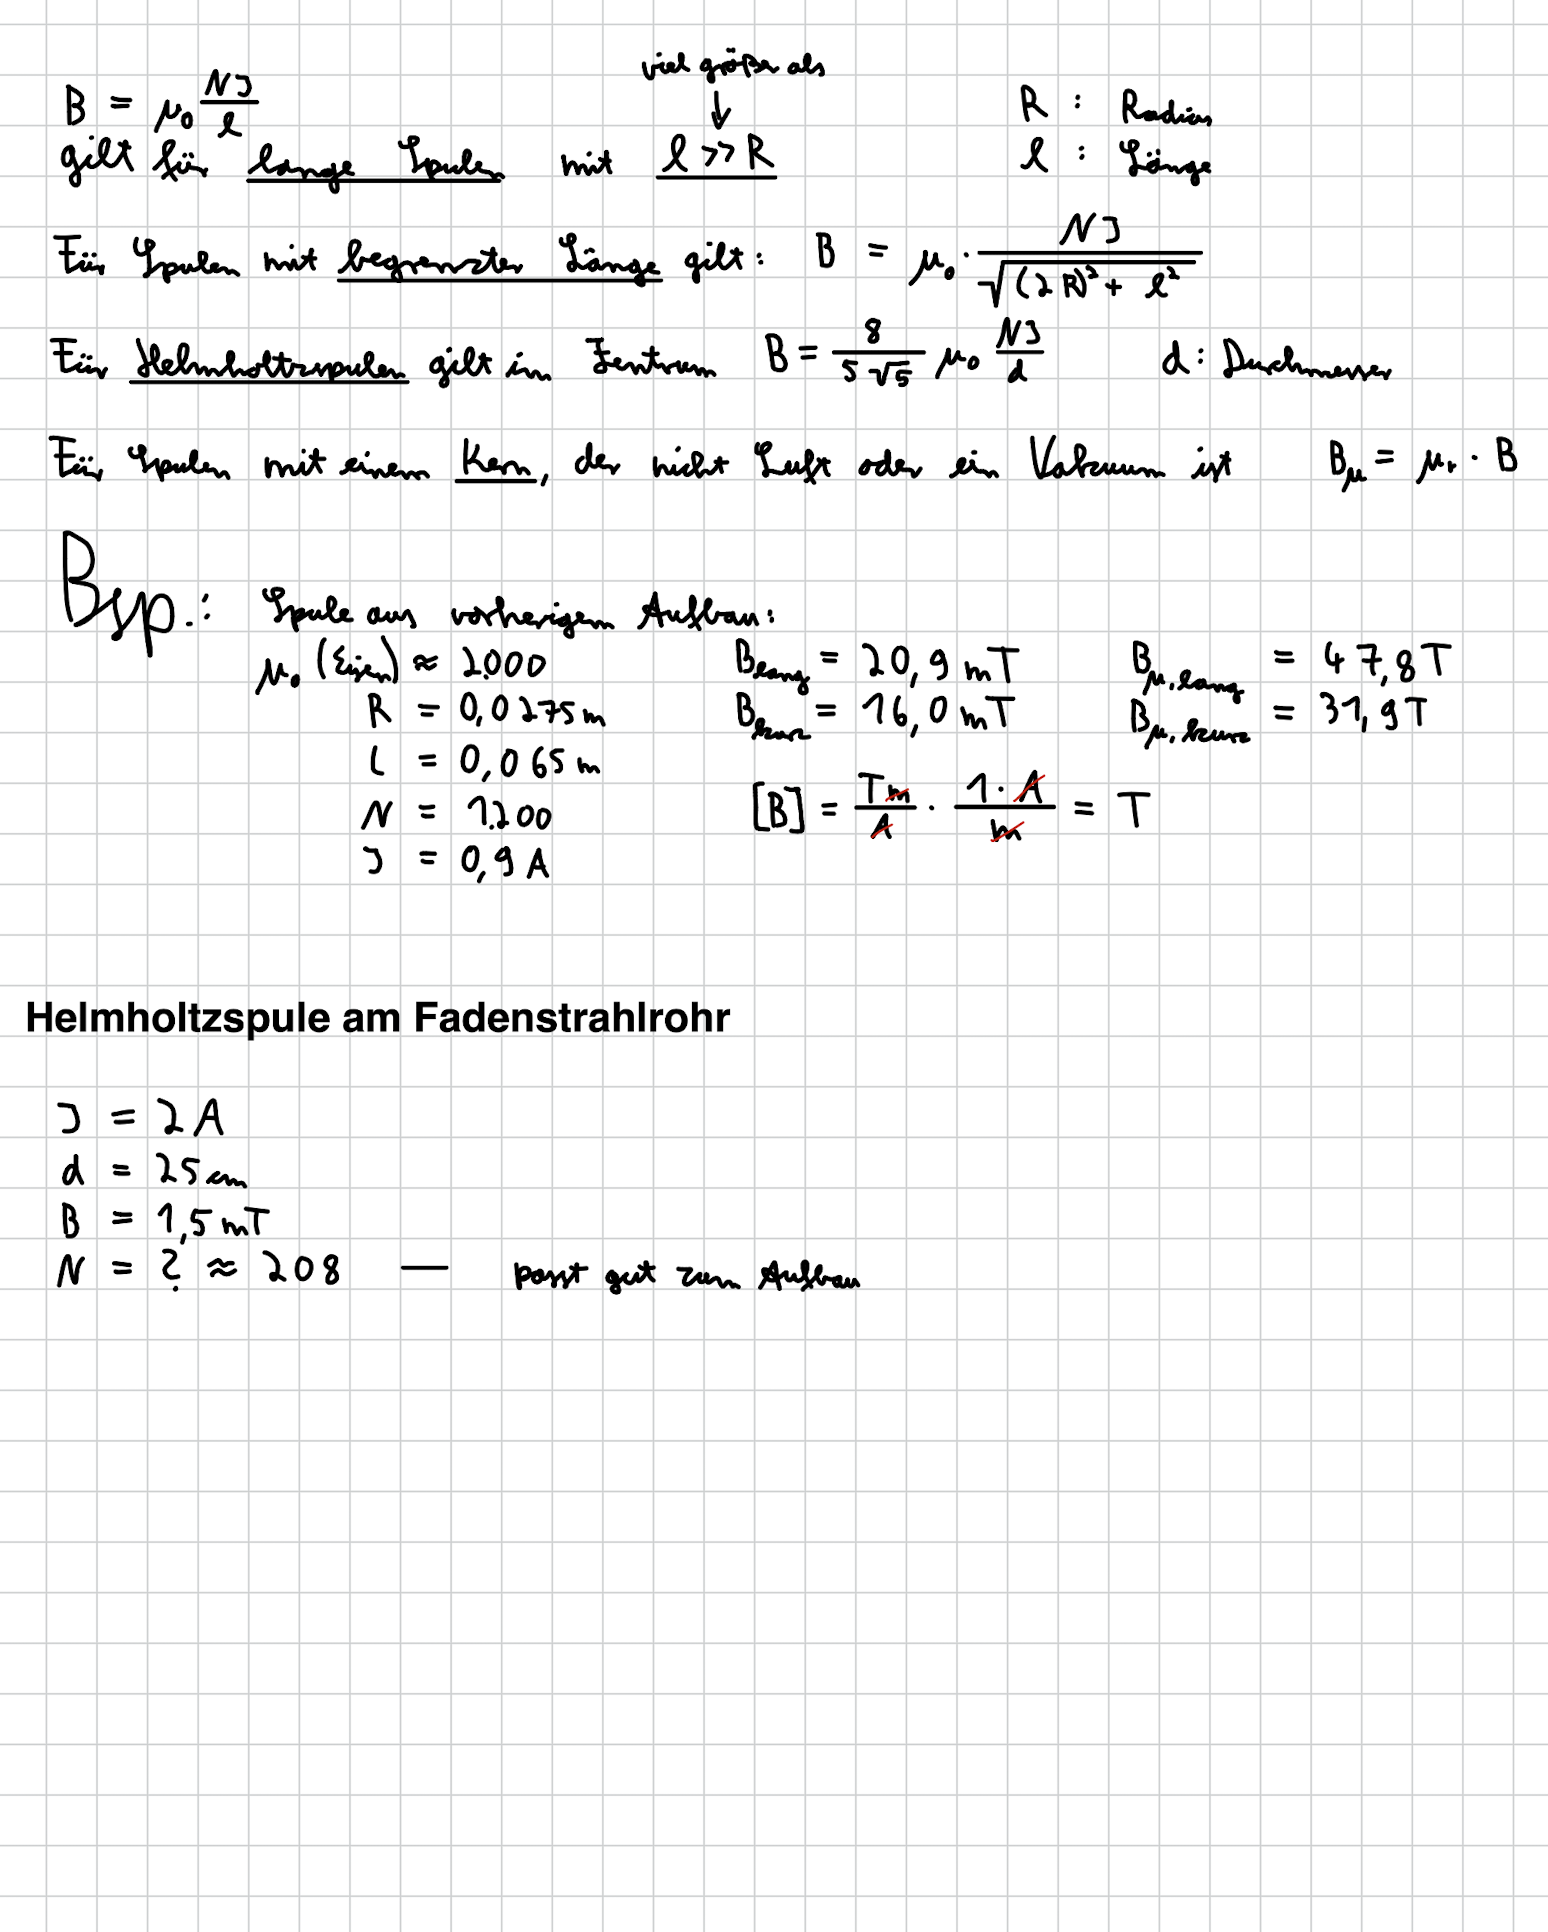
\includegraphics[width=\textwidth]{Images/Magnetfeld einer Spule.png}
	\newpage
	\section{Der magnetische Fluss}
	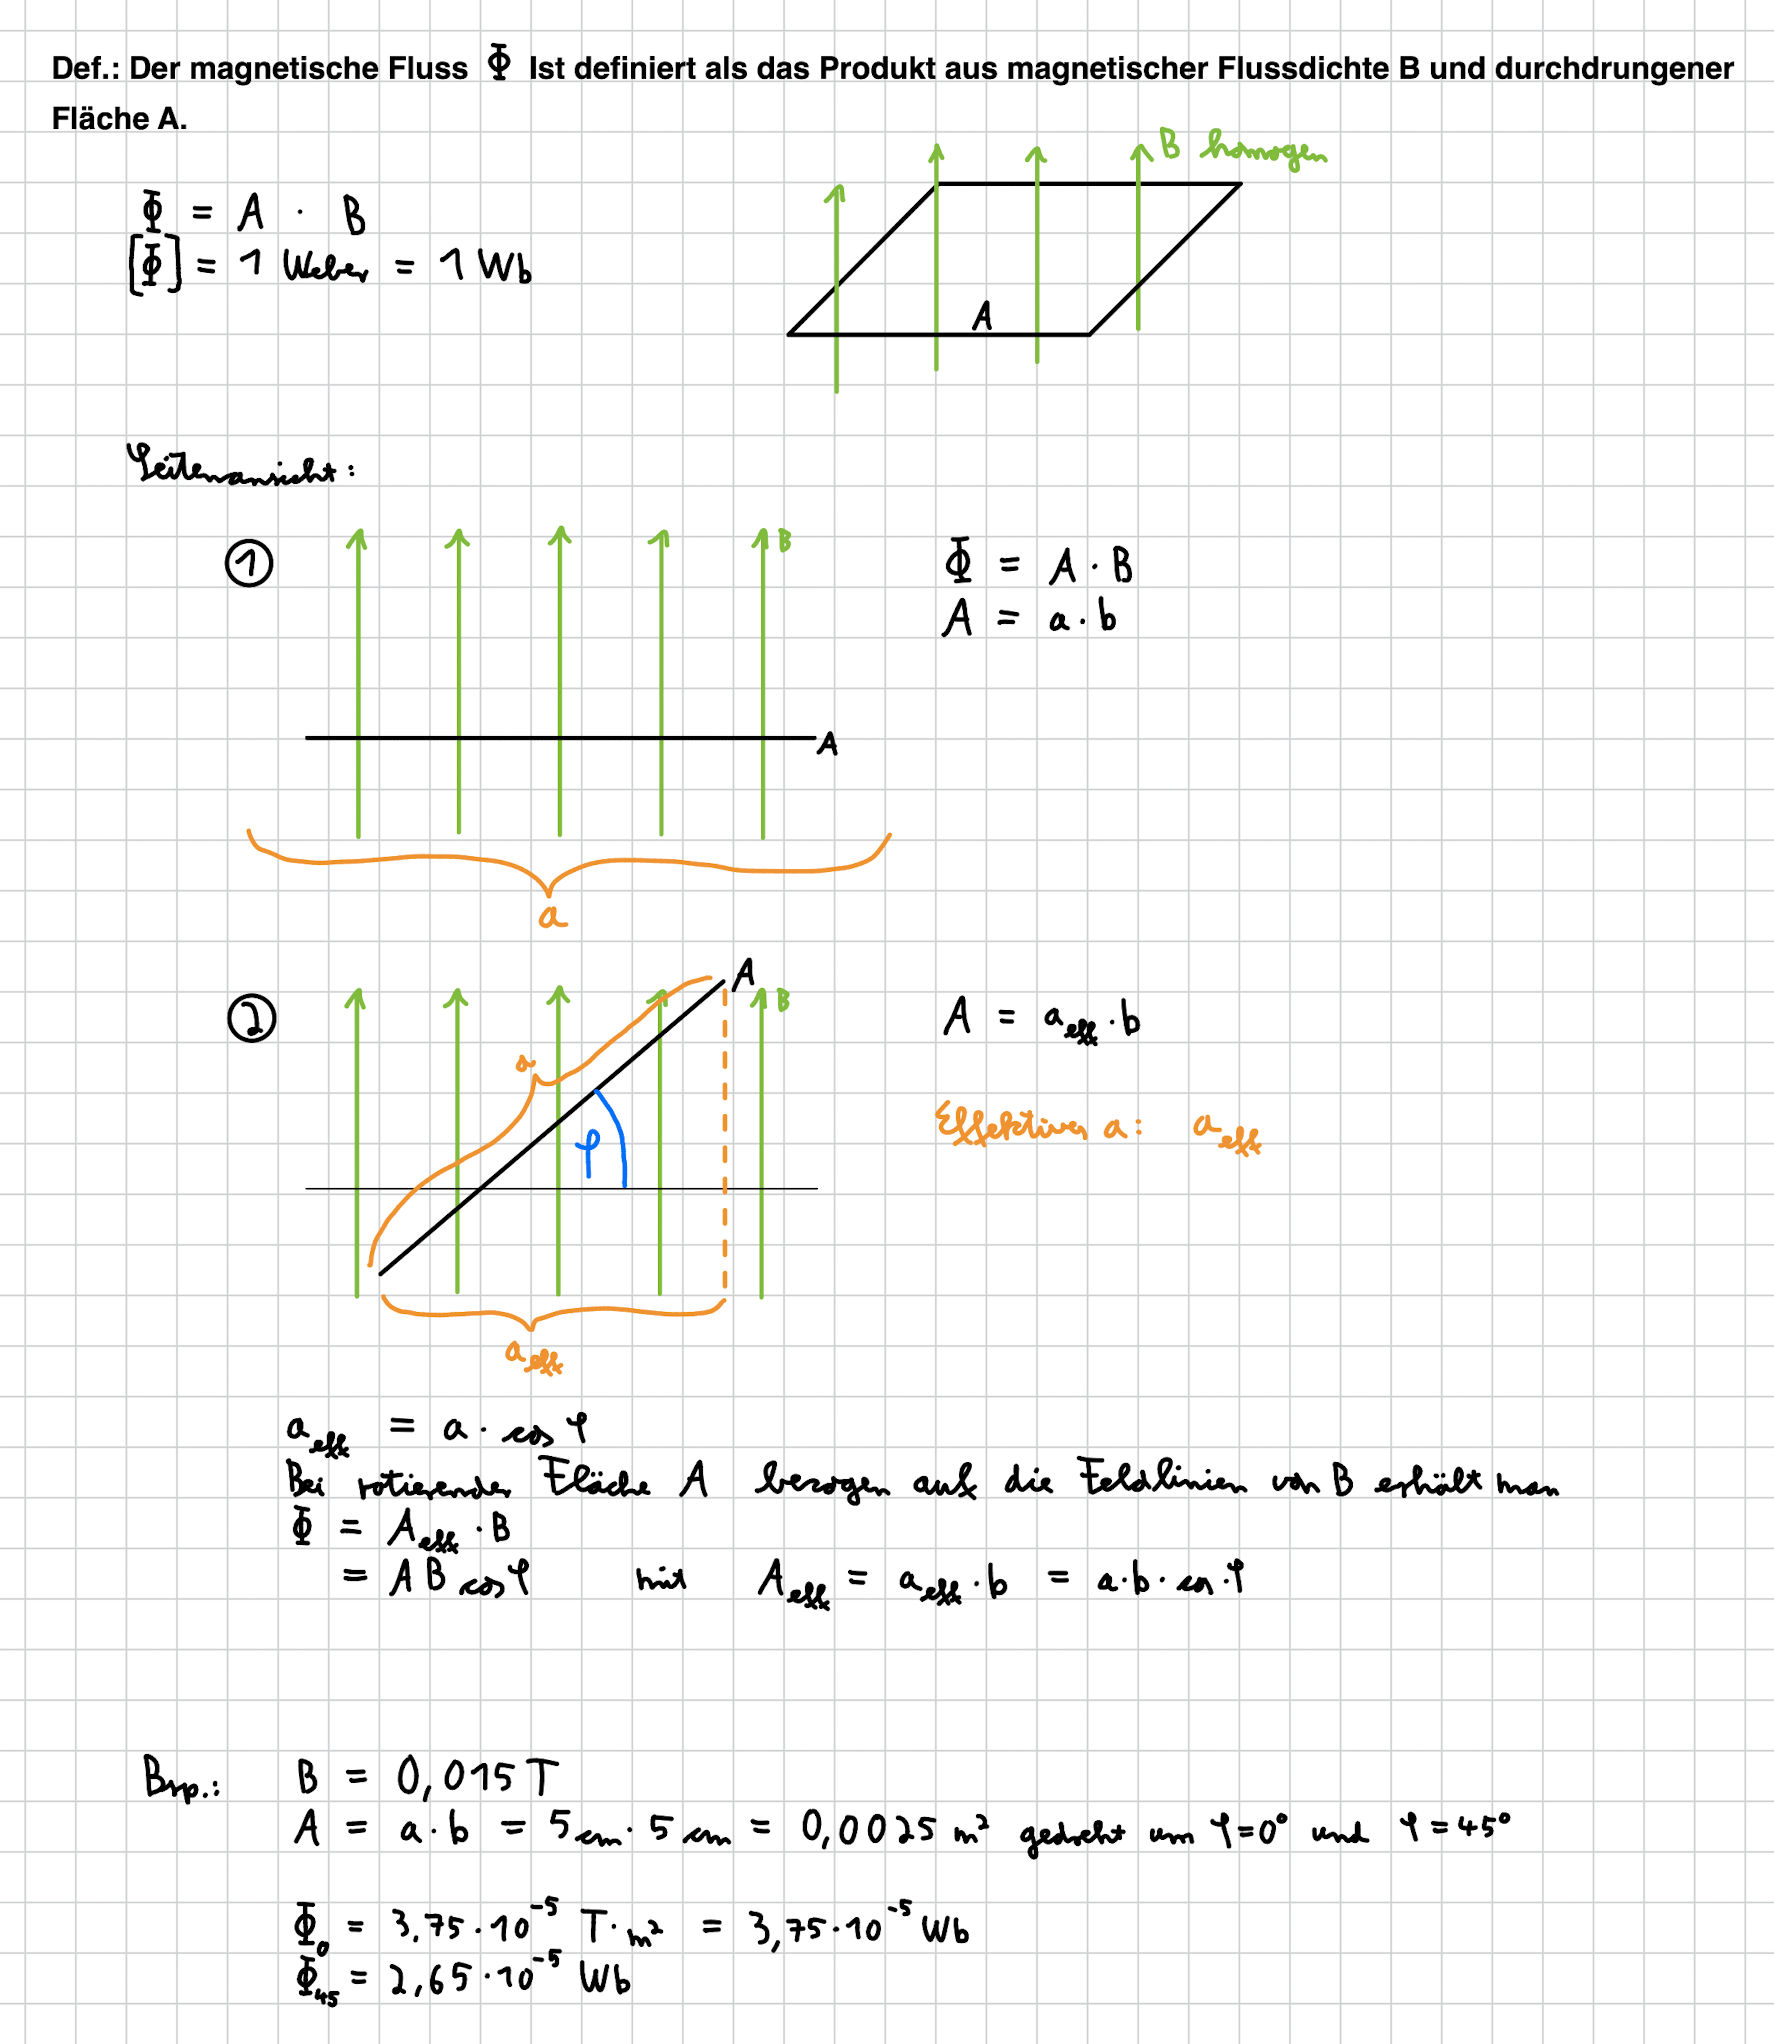
\includegraphics[width=\textwidth]{Images/Der magnetische Fluss.png}
	\newpage
	\section{Elektromagnetische Induktion}
	\textbf{3 Versuche zur Induktion:}
	\\
	\begin{minipage}[t]{0.48\textwidth}
		\vspace{0pt}
		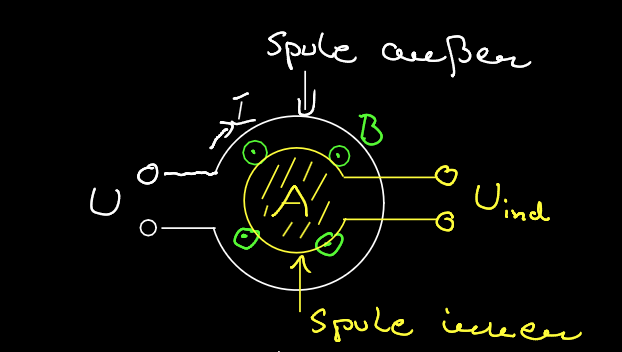
\includegraphics[width=\linewidth]{Images/Elektromagnetische Induktion.png}
	\end{minipage}
	\hfill
	\begin{minipage}[t]{0.48\textwidth}
		\vspace{0pt}
		I dient der Erzeugung eines Magnetfeldes B.\\
		A: Fläche der inneren Spule
		\begin{enumerate}[itemsep=0pt]
			\item Variation von B bewirkt die Erzeugung einer Spannung $U_{ind}$ in der inneren Spule.
			\item Variation von A erzeugt ebenfalls eine Spannung $U_{ind}$.
			\item Rotation der Fläche A im Feld B erzeugt $U_{ind}$.
		\end{enumerate}
	\end{minipage}
	\vspace{0.2cm}
	\\
	$U_{ind}$ wird Induktionsspannung genannt. Sie ist proportional zur Änderung von A und B und damit von $\Phi = A \cdot B$, dem magnetischen Fluss.\\
	Es gilt:
	\begin{alignat}{1}
		U_{ind} &= -N \frac{d \Phi}{dt}\\
		&= - N (\frac{d}{dt} \Phi)\\
		&= -N (\frac{d}{dt} A \cdot B)\\
		&= -N (\frac{d}{dt} A(t) \cdot B(t))\\
		&= -N (\dot{A}B + A \dot{B})\\
	\end{alignat}
	Für A = konst: $U_{ind}  = - NA\dot{B}$\\
	Für B = konst: $U_{ind} = -N B \dot{A}$\\
	\vspace{0.5cm}\\
	\textbf{Bsp.: Rotierende Fläche A}\\
	\begin{minipage}[t]{0.48\textwidth}
		\vspace{0pt}
		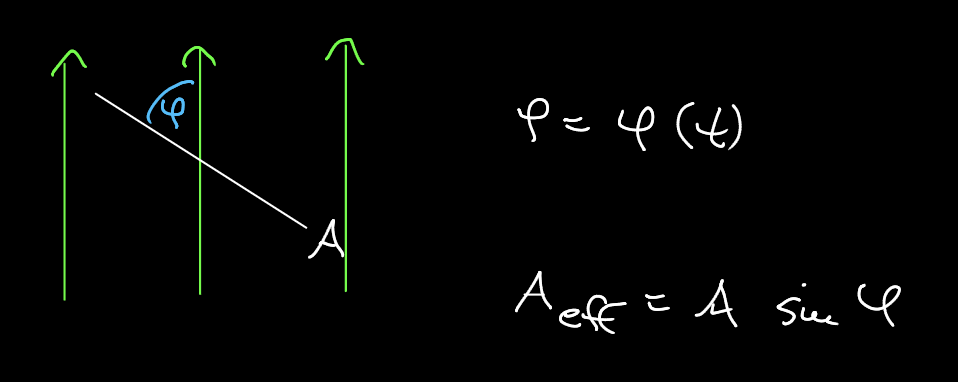
\includegraphics[width=\linewidth]{Images/Elektromagnetische Induktion 2.png}
	\end{minipage}
	\hfill
	\begin{minipage}[t]{0.48\textwidth}
		\vspace{0pt}
		Angenommen, die Fläche A wird f-mal pro Sekunde um sich selbst gedreht.\\
		$\Rightarrow$ f: Rotationsfrequenz\\
		$T = \frac{1}{f}$: Periodendauer\\
	\end{minipage}
	\vspace{0.3cm}\\
	Für den in der Zeit t zurückgelegten Winkel $\varphi$ gilt dann
	\begin{alignat}{1}
		\frac{t}{T} &= \frac{\varphi}{2 \pi} \qquad \mid \cdot 2 \pi\\
		\varphi &= \frac{2 \pi}{T} \cdot t \qquad \mid  \tfrac{2 \pi}{T} = \omega : \text{Winkelgeschwindigkeit}\\
		\Rightarrow A_{eff} &= A \cdot \sin (\omega t)
	\end{alignat}
	\newpage
	\noindent
	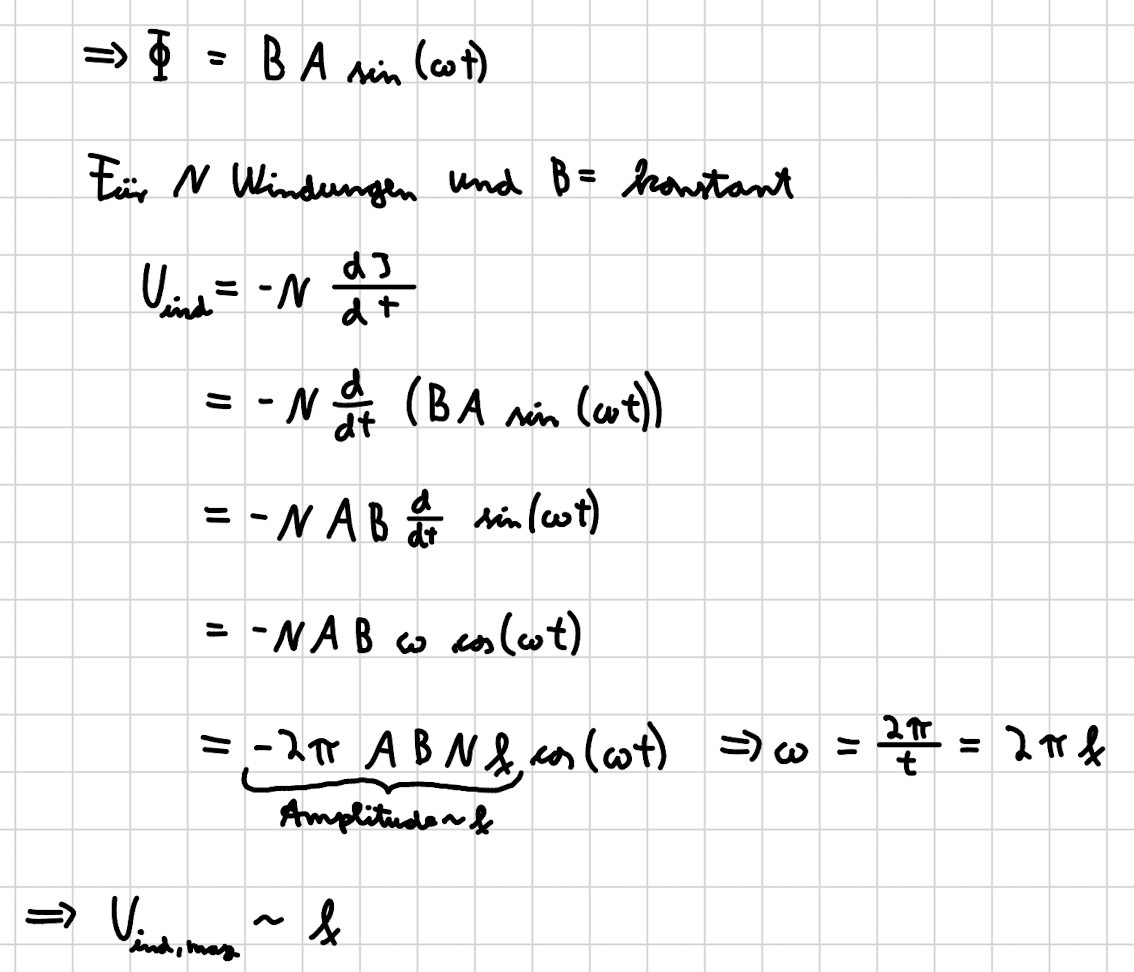
\includegraphics[width=0.4\textwidth]{Images/Elektromagnetische Induktion 3.png}\\
	\\
	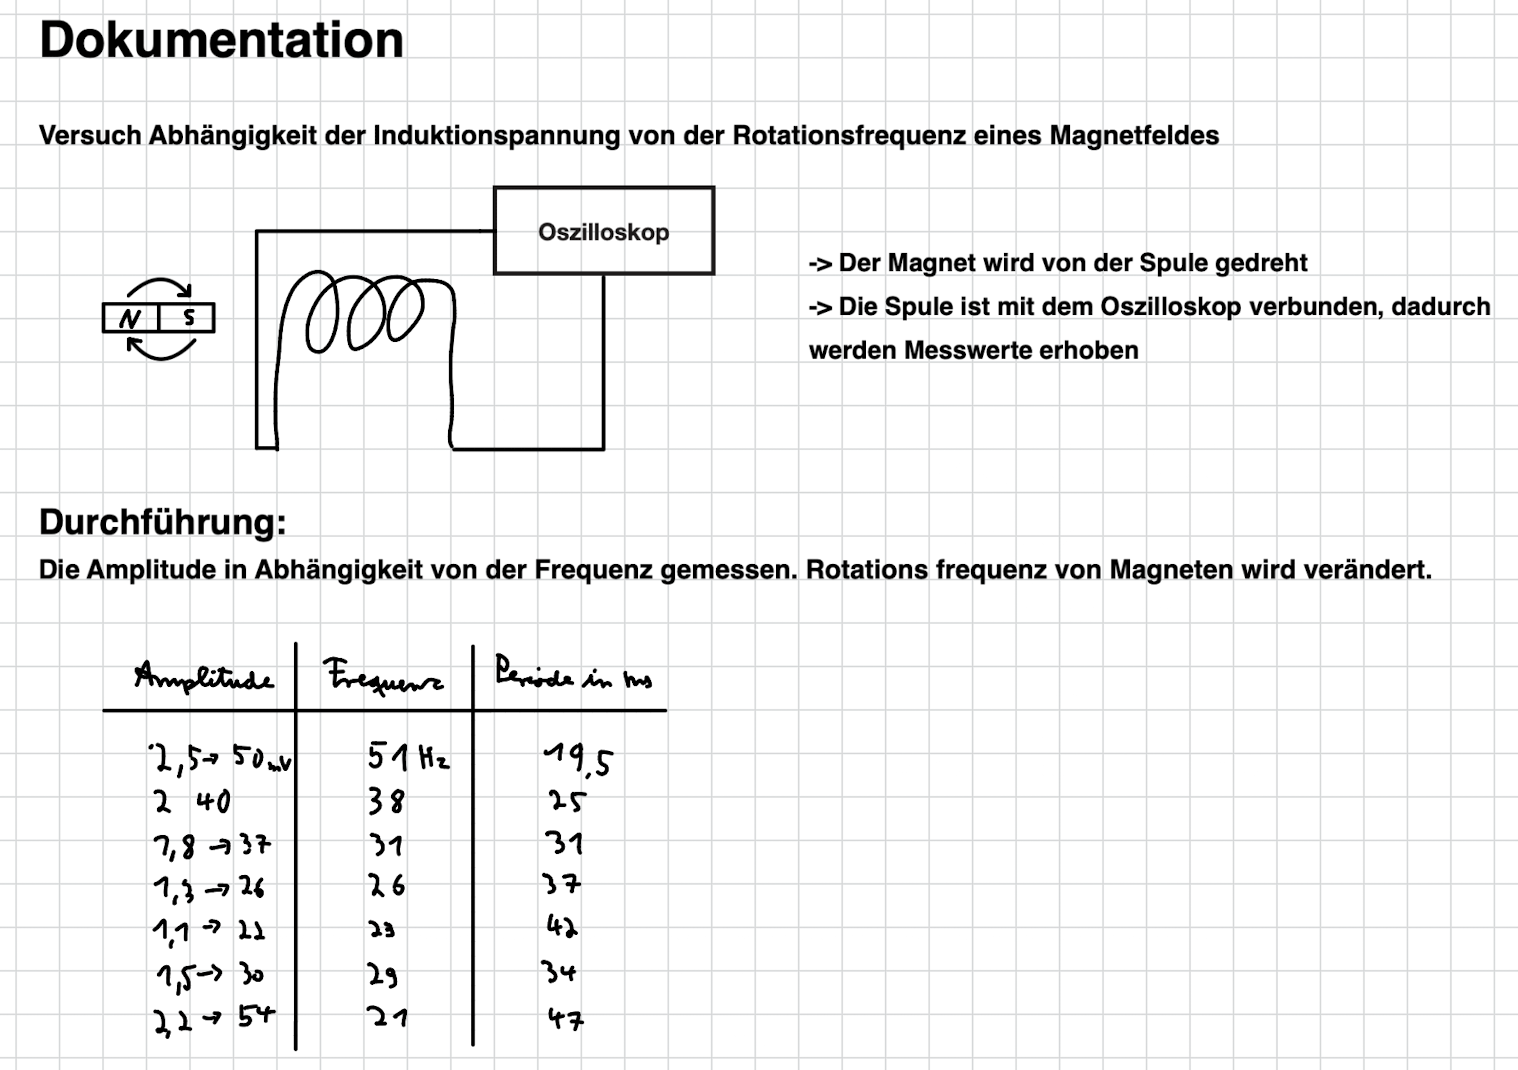
\includegraphics[width=0.8\textwidth]{Images/Elektromagnetische Induktion - Versuch.png}\\
	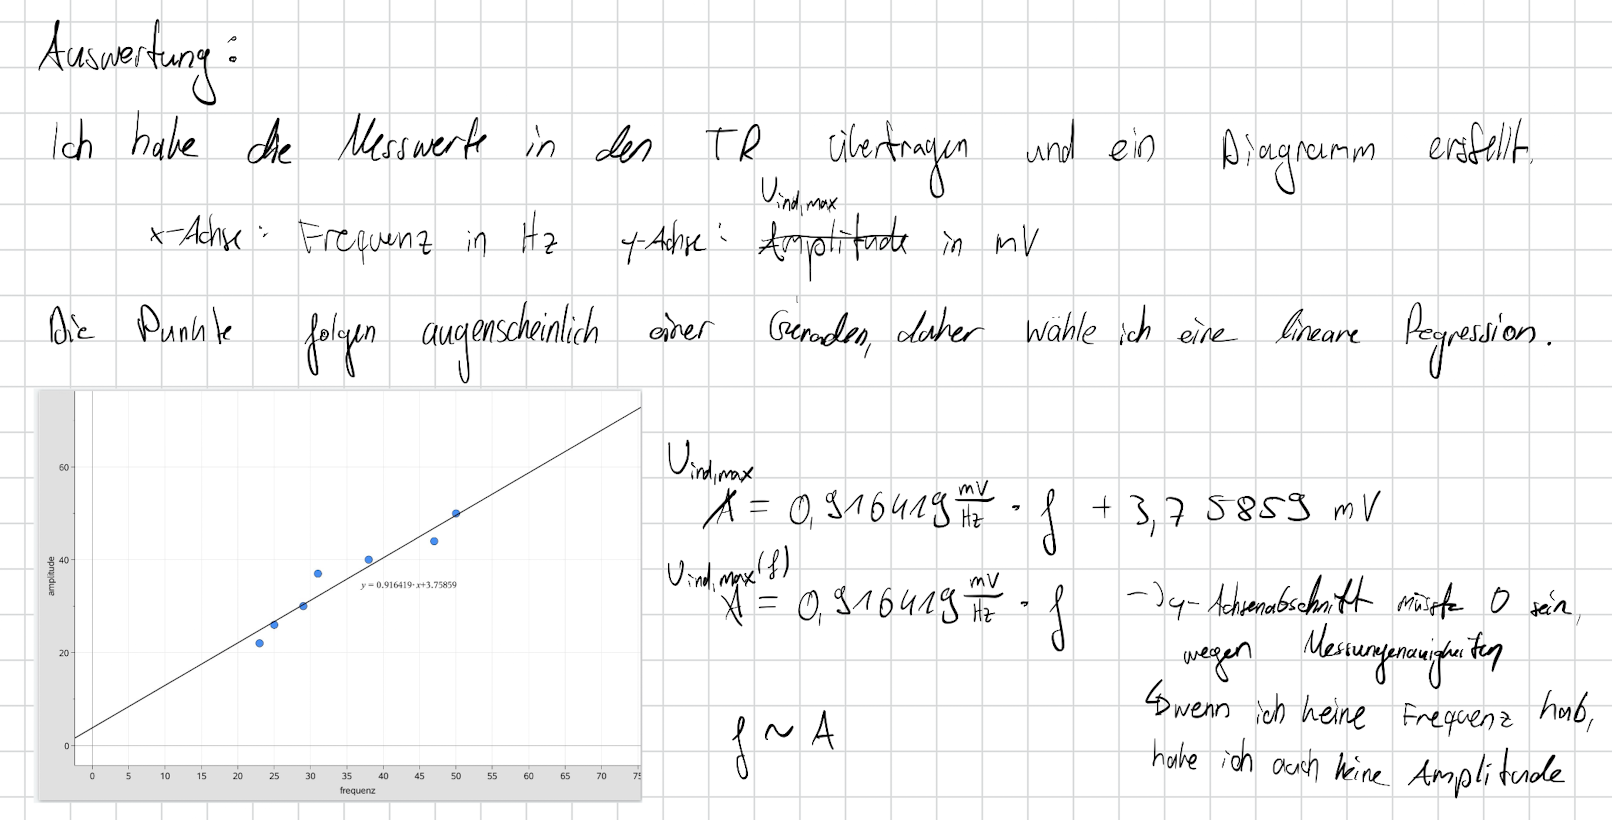
\includegraphics[width=0.8\textwidth]{Images/Elektromagnetische Induktion - Auswertung.png}
	\newpage
	\section{Versuch: Rotation eines Magnetfeldes vor einer Spule}
	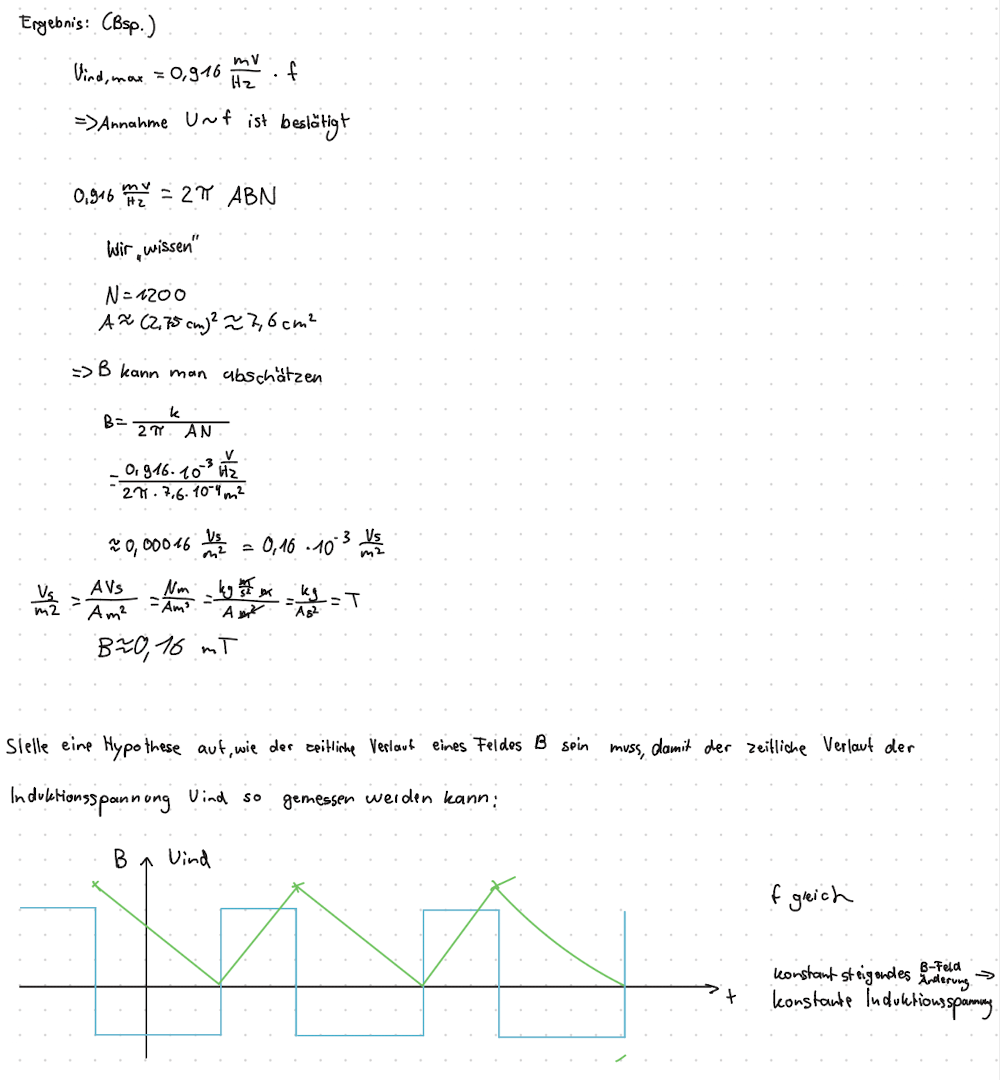
\includegraphics[width=\textwidth]{Images/Elektro.png}
	\newpage
	\section{Die Lenzsche Regel}
	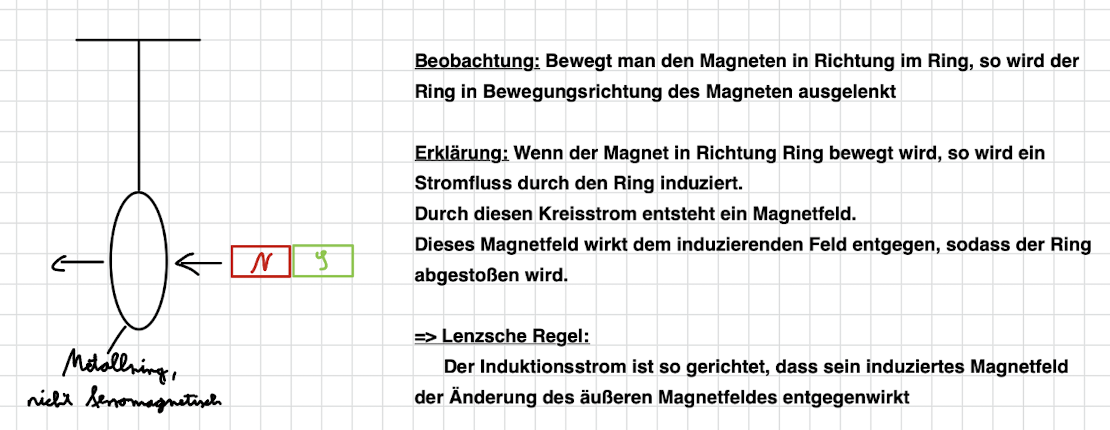
\includegraphics[width=\textwidth]{Images/Die Lenzsche Regel.png}
	\newpage
	\section{Selbstinduktion}
	Legt man an eine Spule eine Spannung an, so baut sich durch den resultierenden Stromfluss in der Spule ein Magnetfeld auf. Dieses sich ändernde Magnetfeld induziert in der Spule eine Induktionsspannung, die dem sich ändernden Stromfluss entgegenwirkt.
	

	\begin{align*}
		U_{\text{ind}} 
		&= -N \frac{d\Phi}{dt}
		&& B \sim I\text{ (homogenes Feld)} \\
		&= -N A \frac{dB}{dt} 
		&& B = k*I \quad \mid \quad \text{\textbf{k}: Spuleneigenschaften}\\
		&= -N A k \frac{dI}{dt}
		&&L := N A k \quad \mid \quad \text{\textbf{L}: Induktivität der Spule}
	\end{align*}
	\begin{align*}
		\qquad  U_{ind} \sim \dot{I} \quad \Rightarrow \quad U_{\text{ind}} = -L \dot I\\
		[L] = 1 \frac{Vs}{A} = 1 \text{ Henry}= 1 H
	\end{align*}
	\vspace{0.5cm}
	Die Selbstinduktionsspannung $U_{L}$ wirkt der Änderung des Stromflusses entgegen $U_L = -U_{ind} = L\dot{I}$
	
	
	\begin{figure}[htbp]
		\centering
		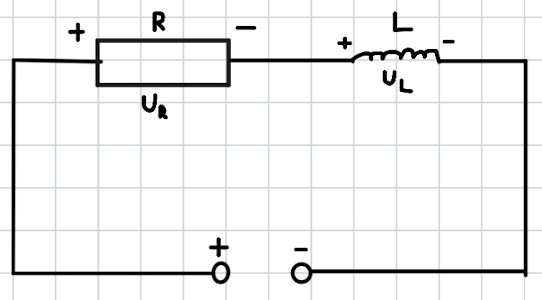
\includegraphics[width=0.6\linewidth]{Images/Schaltplan Selbstinduktion}
		\caption{Schaltplan}
	\end{figure}
	
	
	\newpage
	\section{Ladekurve einer Induktivität}
	
	\vspace{0.5cm}
	
	\begin{center}
		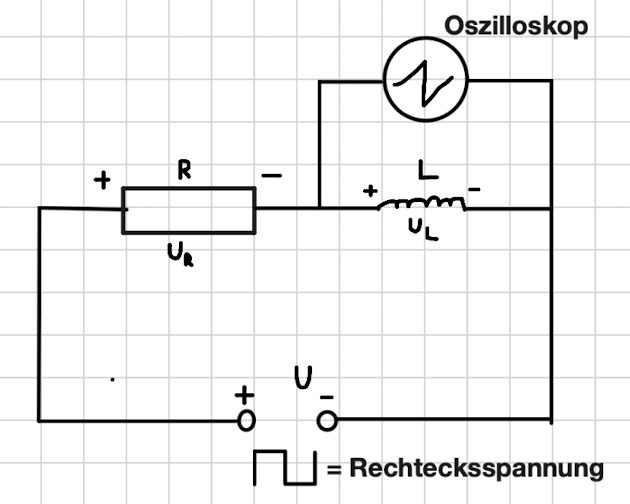
\includegraphics[width=0.5\linewidth]{Images/Schaltplan Induktivität}
	\end{center}
	
	\vspace{0.5cm}
	
	\begin{figure}[h]
		\centering
		\begin{minipage}{0.48\textwidth}
			Beim \textbf{Einschaltvorgang} (Spannung $U$ von 0\,V auf $U_0$) erhält man folgende Kurve auf dem Oszilloskop:
		\end{minipage}
		\hfill
		\begin{minipage}{0.48\textwidth}
			Das Bild beim \textbf{Ausschaltvorgang} ist:
		\end{minipage}
		
		\vspace{0.5cm}
		
		\begin{minipage}{0.4\textwidth}
			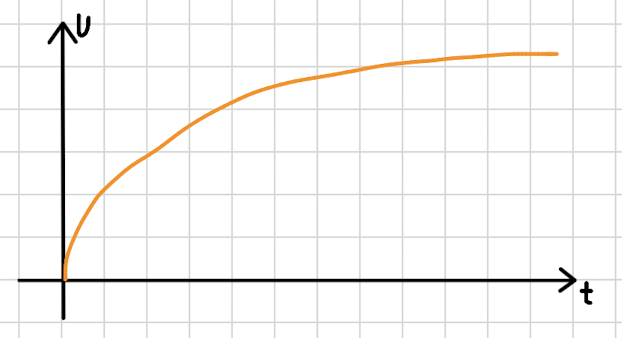
\includegraphics[width=\linewidth]{Images/Ladekurve Oszilloskop}
		\end{minipage}
		\hfill
		\begin{minipage}{0.4\textwidth}
			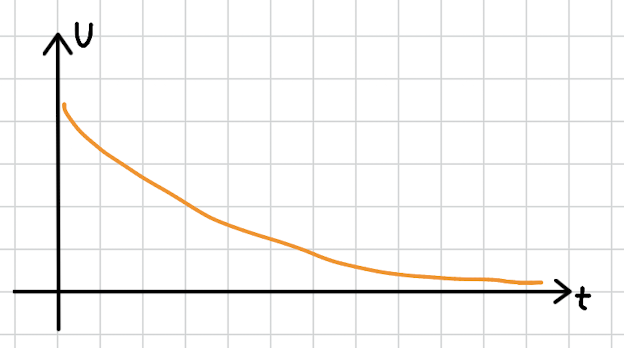
\includegraphics[width=\linewidth]{Images/Entladekurve Oszilloskop}
		\end{minipage}
		
		\vspace{0.5cm}
		\begin{minipage}{0.6\textwidth}
			\begin{align}
				U_L + U_R - U_0 &= 0 \\
				U_L + U_R &= U_0 \\
				L\dot I + RI &= U_0  \quad &&| - RI \\
				L\dot I &= U_0 - RI && | : L \\
				\dot I &= \frac{U_0}{L} - \frac{R}{L} I  &&\Rightarrow \text{Substitution: } K
			\end{align}
			\begin{align}
				\frac{dK}{dI} &= - \frac{R}{L}\\
				dI &= - \frac{L}{R} dK\\
				\dot{I} &= \frac{dI}{dt} = - \frac{L}{R} \frac{dK}{dt} = K \qquad && | KW \\
				-\frac{R}{L} \frac{dt}{dK} &= \frac{1}{K} \qquad &&| *dK\\
				-\frac{R}{L} dt &= \frac{1}{K} * dK
			\end{align}
		\end{minipage}
		\hfill
		\begin{minipage}{0.4\textwidth}
			
		\end{minipage}
	\end{figure}
	
	\newpage
	\begin{align}
		- \frac{R}{L} \int_0^t  d\tilde{t} &= \int_{K_0}^K  \frac{1}{\tilde{K}} d \tilde{K}\\
		- \frac{R}{L} \Big[\tilde{t} \Big]_0^t &= \big[\ln \tilde{K}\big]_{K_0}^K\\
		e^{- \frac{R}{L} \cdot t} &= \frac{K}{K_0}
	\end{align}
	\subsubsection*{Rücksubstitution}
	\begin{align}
		\frac{K}{K_0} &= \frac{\frac{U_0}{L} - \frac{R}{L} \cdot I} 
		{\frac{U_0}{L} - \frac{R}{L} \cdot I_0}
		&&\mid \textbf{Einschalten: } I_0 = I (t=0) = 0\\
		&=\frac{\frac{U_0}{L} - \frac{R}{L} \cdot I}{\frac{U_0}{L} }\\
		&= \frac{U_0 - RI}{U_0} = 1 - \frac{RI}{U_0} = e^{- \frac{R}{L} \cdot t}\\
		\frac{RI}{U_0} &= 1 - e^{- \frac{R}{L} \cdot t}
		&&\mid \cdot \frac{U_0}{R}\\
		I(t) &= \frac{U_0}{R} \left(1 - e^{- \frac{R}{L} \cdot t}\right)
	\end{align}
	\begin{align}                                                                                                                                      
      U_L + U_R &= 0                                                                                                                                 
          && \leftarrow \text{Keine Spannung von außen}\\[6pt]                                                                                       
      L \dot{I} + RI &= 0
          && \mid {-RI} \mid {:L}\\                                                                                                                  
      \dot{I} &= -\frac{R}{L} I\\[6pt]
      \frac{dI}{dt} &= - \frac{R}{L} I                                                                                                               
          && \mid {\cdot\, dt} \mid {:I}\\[6pt]                                                                                                      
      \int_{I_{max}}^{I} \frac{1}{\tilde{I}} d \tilde{I}
          &= - \frac{R}{L} \int_{0}^{t} d \tilde{t}                                                                                                  
          && \left(\frac{d \tilde{I}}{\tilde{I}} = \frac{1}{\tilde{I}} d \tilde{I}\right)\\[4pt]
      \Big[\ln \tilde{I} \Big]_{I_{max}}^{I}                                                                                                         
          &= - \frac{R}{L} \Big[\tilde{t}\Big]_0^t\\[6pt]                                                                                            
      \frac{I}{I_{max}} &= e^{- \frac{R}{L} t}\\[4pt]                                                                                                
      I(t) &= I_{max} e^{- \frac{R}{L} t} = I_{max} e^{- \frac{t}{\tau}}\\[8pt]                                                                      
      \text{Lebensdauer: } \tau
          &= \frac{1}{\frac{R}{L}} = \frac{L}{R}\\[4pt]                                                                                              
      \text{Test: } \Big[\frac{L}{R}\Big]
          &= \frac{\frac{Vs}{A}}{\frac{V}{A}} = \frac{Vs}{A} \cdot \frac{A}{V} = s\\[8pt]                                                                                                  
      \Rightarrow\; t_{1/2} &= \ln 2 \cdot \tau
          && \mid \ln\\[4pt]                                                                                                                         
      \Leftrightarrow\; e^{- \frac{t}{\tau}}                                                                                                         
          &= 2^{- \frac{t}{t_{1/2}}} \ln 2
          && \text{t = 0 irrelevant}\\[4pt]                                                                                                          
      \Rightarrow\; - \frac{1}{\tau}                                                                                                                 
          &= - \frac{\ln 2}{t_{1/2}}
          && \mid \cdot (-1) \mid \cdot \tau \mid \cdot t_{1_{1/2}}\\[4pt]                                                                           
      \Leftrightarrow\; t_{1/2} &= \ln 2 \cdot \tau                                                                                                  
	\end{align}
  	\newpage
	
	\section{Energie im magnetischen Feld einer Induktivität}
	\begin{align}
		E &= \int_{0}^{\infty} P(t) \cdot dt\\
		&= \int_{0}^{\infty} I(t) \cdot U_L (t) dt
		&& I(t) = I_{max}  \Big (1 - e^{- \frac{R}{L} t} \Big )
	\end{align}
	\begin{align}
		U_R + U_L &= U_0\\
		IR + U_L &= U_0 = I_{max} R \qquad \mid - IR\\
		U_L &= I_{max} R - I R\\
		&= I_{max} R - I_{max} R (1 - e^{- \frac{R}{L} t})\\
		&= I_{max} R - I_{max} R + I_{max} R - I_{max} R  e^{- \frac{R}{L} t}\\
		&= I_{max} R e^{- \frac{R}{L} t}
	\end{align}
	\begin{align}
		E &= \int_{0}^{\infty} I_{max} (1 - e^{- \frac{R}{L} t}) \cdot I_{max} R e^{-\frac{R}{L} t} dt\\
		&= \int \Big (I_{max}^2 R e^{- \frac{R}{L} t} - I_{max}^2 R
		\cdot e^{- \frac{R}{L} t}\cdot e^{- \frac{R}{L} t} \Big ) dt\\
		&= I_{max}^2 R \int_{0}^{\infty} \Big (e^{- \frac{R}{L} t} - e^{-2 \frac{R}{L} t} \Big) dt\\
		&= I_{max}^2 R \Big [- \frac{L}{R} e^{- \frac{R}{L} t} +
		\frac{L}{2R} e^{-2 \frac{R}{L} t}\Big]_0^\infty\\
		&= I_{max}^2 R \Big (\frac{L}{R} - \frac{1}{2} \frac{L}{R} \Big) \\
		&= I_{max}^2 R \cdot \frac{1}{2} \frac{L}{R}\\
		&= \frac{1}{2} L I_{max}^2 && \mid R = \frac{U}{I} 
		\qquad \text{\textbf{L}: Proportionalitätskonstante}\\
		&= \frac{1}{2} \cdot \frac{L}{R^2} U_0^2
		&& \mid I_{max} = \frac{U_0}{R}
	\end{align}
	
	\vspace{0.5cm}
	
	\subsection*{Aufgabe}

	\begin{minipage}[t]{0.48\textwidth}
		\begin{tabular}{|c|c|c|c|c|c|}
		\hline
		t (ms) & 20 & 40 & 60 & 80 & 100\\
		\hline
		I (A) & 0.068 & 0.047 & 0.031 & 0.02 & 0.013\\
		\hline
		\end{tabular}\\
		\\
		\textbf{Messung mit R = 100 $\Omega$\\
		Bestimme I(t), L, E}
	\end{minipage}
	\hfill
	\begin{minipage}[t]{0.4\textwidth}
		\begin{align}
		b^t &= e^{- \frac{t}{\tau}} \qquad \mid \ln \\
		\Leftrightarrow t \ln b &= - \frac{t}{\tau} \\
		\Leftrightarrow \tau &= - \frac{1}{\ln b} = \frac{L}{R}
		\end{align}		
	\end{minipage}
	

	\newpage
	\textbf{I(t):}
	\begin{itemize}
		\item Werte in Tabelle in TR übernehmen.
		\item Diagramm anlegen.\\
		- x-Achse: t(ms)\\
		- y-Achse: I(A)
		\item Die Punkte verlaufen augenscheinlich entlang dem Graphen einer Exponentialfunktion.\\
		$\Rightarrow$ Exponentielle Regression $I(t) = 0.106 \cdot 0.979^x \overset{!}{=} 0.106 \cdot e^{- \frac{x}{\tau}}$
		\vspace{0cm}
		\begin{alignat}{3}
			&\Leftrightarrow \hspace{1cm}
			& 0{,}979^x  &= e^{-\frac{x}{\tau}} &\hspace{1.5cm} &\mid \ln \\
			&\Leftrightarrow & x \ln 0{,}979  &= -\frac{x}{\tau} \\
			&	\underset{x \neq 0}{\Leftrightarrow} & \ln 0{,}979    &= -\frac{1}{\tau}  &\qquad & x \neq 0 \\
			&\Leftrightarrow & \tau &= -\frac{1}{\ln 0{,}979} &\qquad &\rightarrow \text{In der Arbeit statt „0,979“ „Stat.b“ einfügen} \\
			&\Rightarrow & \tau &= 48{,}036
		\end{alignat}
		Die Lebensdauer beträgt $\tau = 48ms$. 
		$R = 100 \Omega$
		\begin{align}
			\tau = \frac{L}{R} \Leftrightarrow L &= \tau R\\
			&= 48 \cdot 10^{-3} \cdot1 \cdot 10^2 \Omega s \\
			&= 4,8 H\\ 
			I (t) &= 0,106 A \cdot e^{- \frac{t}{48ms}}\\
			E &= \frac{1}{2} L I^2_{max}\\
			&= \frac{1}{2} \cdot 4,8H \cdot (0,106 A)^2\\
			&= 0,027 J
		\end{align}
	\end{itemize}
	
	\subsection{Beispielaufgaben:}
	\begin{minipage}[t]{0.48\textwidth}
		\textbf{1) } Zeichne den Schaltplan zur Bestimmung der Ausschaltspannung an einer Spule
		\begin{tikzpicture}[circuit ee IEC]
			\hspace{2.cm}
			\draw (0,1) to[resistor={info=$R$}] (2,1)
			to[inductor={info=$L$}] (4, 1) 
			-- (4,0) -- (0,0) -- (0,1)
			(2,1) node[contact] {} --
			(2,2) to[voltmeter={info=$U$}] (4,2) -- (4,1)
			node[contact] {};
		\end{tikzpicture}
	\end{minipage}
	\hfill
	\begin{minipage}[t]{0.48\textwidth}
		\textbf{2) }
		Bestimme die DGL zur Beschreibung des Stromflusses I in der Schaltung
		\begin{align}
			\hspace{2.5cm} U_R + U_L &= 0 \\
			U_R &= RI \\
			U_L &= L \dot{I}\\
			\rightarrow RI + L\dot{I} &= 0
		\end{align}
	\end{minipage}
	\vspace{0.5cm}\\
	\textbf{3) }
	Überprüfe, ob die Funktion $I (t) = I_{max} e^{- \frac{R}{L} t}$ die DGL löst\\
	$\dot{I} (t) = I_{max} \big ( - \frac{R}{L} \big ) e^{- \frac{R}{L} t}$\\
	Einsetzen:
	\begin{alignat}{1}
		R I_{max} e^{- \frac{R}{L} t} - L \tfrac{R}{L} I_{max} e^{- \frac{R}{L} t} &= 0 \qquad \mid
		: e^{- \frac{R}{L} t}\\
		RI_{max} - RI_{max} &= 0\\ 
		0 &= 0
	\end{alignat}
	
	\section{Übung für die Arbeit}
	\subsection{Entladekurve im Kondensator}
	\textbf{Aufgabe:}\\
	Finde $\tau$ heraus - Wann die Spannung null ist.\\
	\begin{minipage}[t]{0.28\textwidth}
		\begin{alignat}{1}
			U_0 &= 4V\\
			R &= 22000 \Omega \\
			C &= 100nF\\
			t(s) &= 10\\
			I (mA) &= 1.77\\
		\end{alignat}
	\end{minipage}
	\hfill
	\begin{minipage}[htbp]{0.68\textwidth}
		\begin{tabular}{|c|c|c|c|c|c|}
			\hline t(s) & 0.001 & 0.002 & 0.003 & 0.004 & 0.005\\
			\hline I($\mu$A) & 115 & 73 & 46 & 30 & 19\\
			\hline
		\end{tabular}
	\end{minipage}
	\begin{alignat}{1}
		y&= 179.291 \cdot \Big(9.7947 \cdot 10^{-196}\Big)^x\\
		\Big(9.7947 \cdot 10^{-196}\Big)^{\frac{t}{1s}} &= e^{- \frac{t}{\tau}} \qquad \mid \ln\\
		\Leftrightarrow \frac{t}{1s} \ln (9.7947 \cdot 10^{-196}) &= - \frac{t}{\tau} \qquad \mid \tau\\
		\Leftrightarrow \tau \cdot \ln \Big(9.7947 \cdot 10^{-196}\Big) \cdot \frac{t}{1s} &= -t \qquad \mid : t\\
		\Leftrightarrow \tau \cdot \ln \Big(9.7947 \cdot 10^{-196}\Big) \cdot \frac{1}{1s} &= -1 \qquad \mid : \Big( \ln(...)\cdot \frac{1}{1s} \Big)\\
		\Leftrightarrow \tau &= - \frac{1}{\ln (9.7947 \cdot 10^{-196})}	 \cdot 1s = 2.2ms\\
	\end{alignat}
	\begin{alignat}{1}
		R &= 22000 \Omega\\
		\tau &= RC\\
		C &= \frac{\tau}{R} = \frac{0.0022s}{22000\Omega} = \frac{0.0001}{10000} F = 1 \cdot 10^{-7} F = 100nF\\
	\end{alignat}
	
	\subsection{Ablesen und interpretieren eines Oszilloskopbildes}
	\vspace{0.5cm}
	\begin{center}
		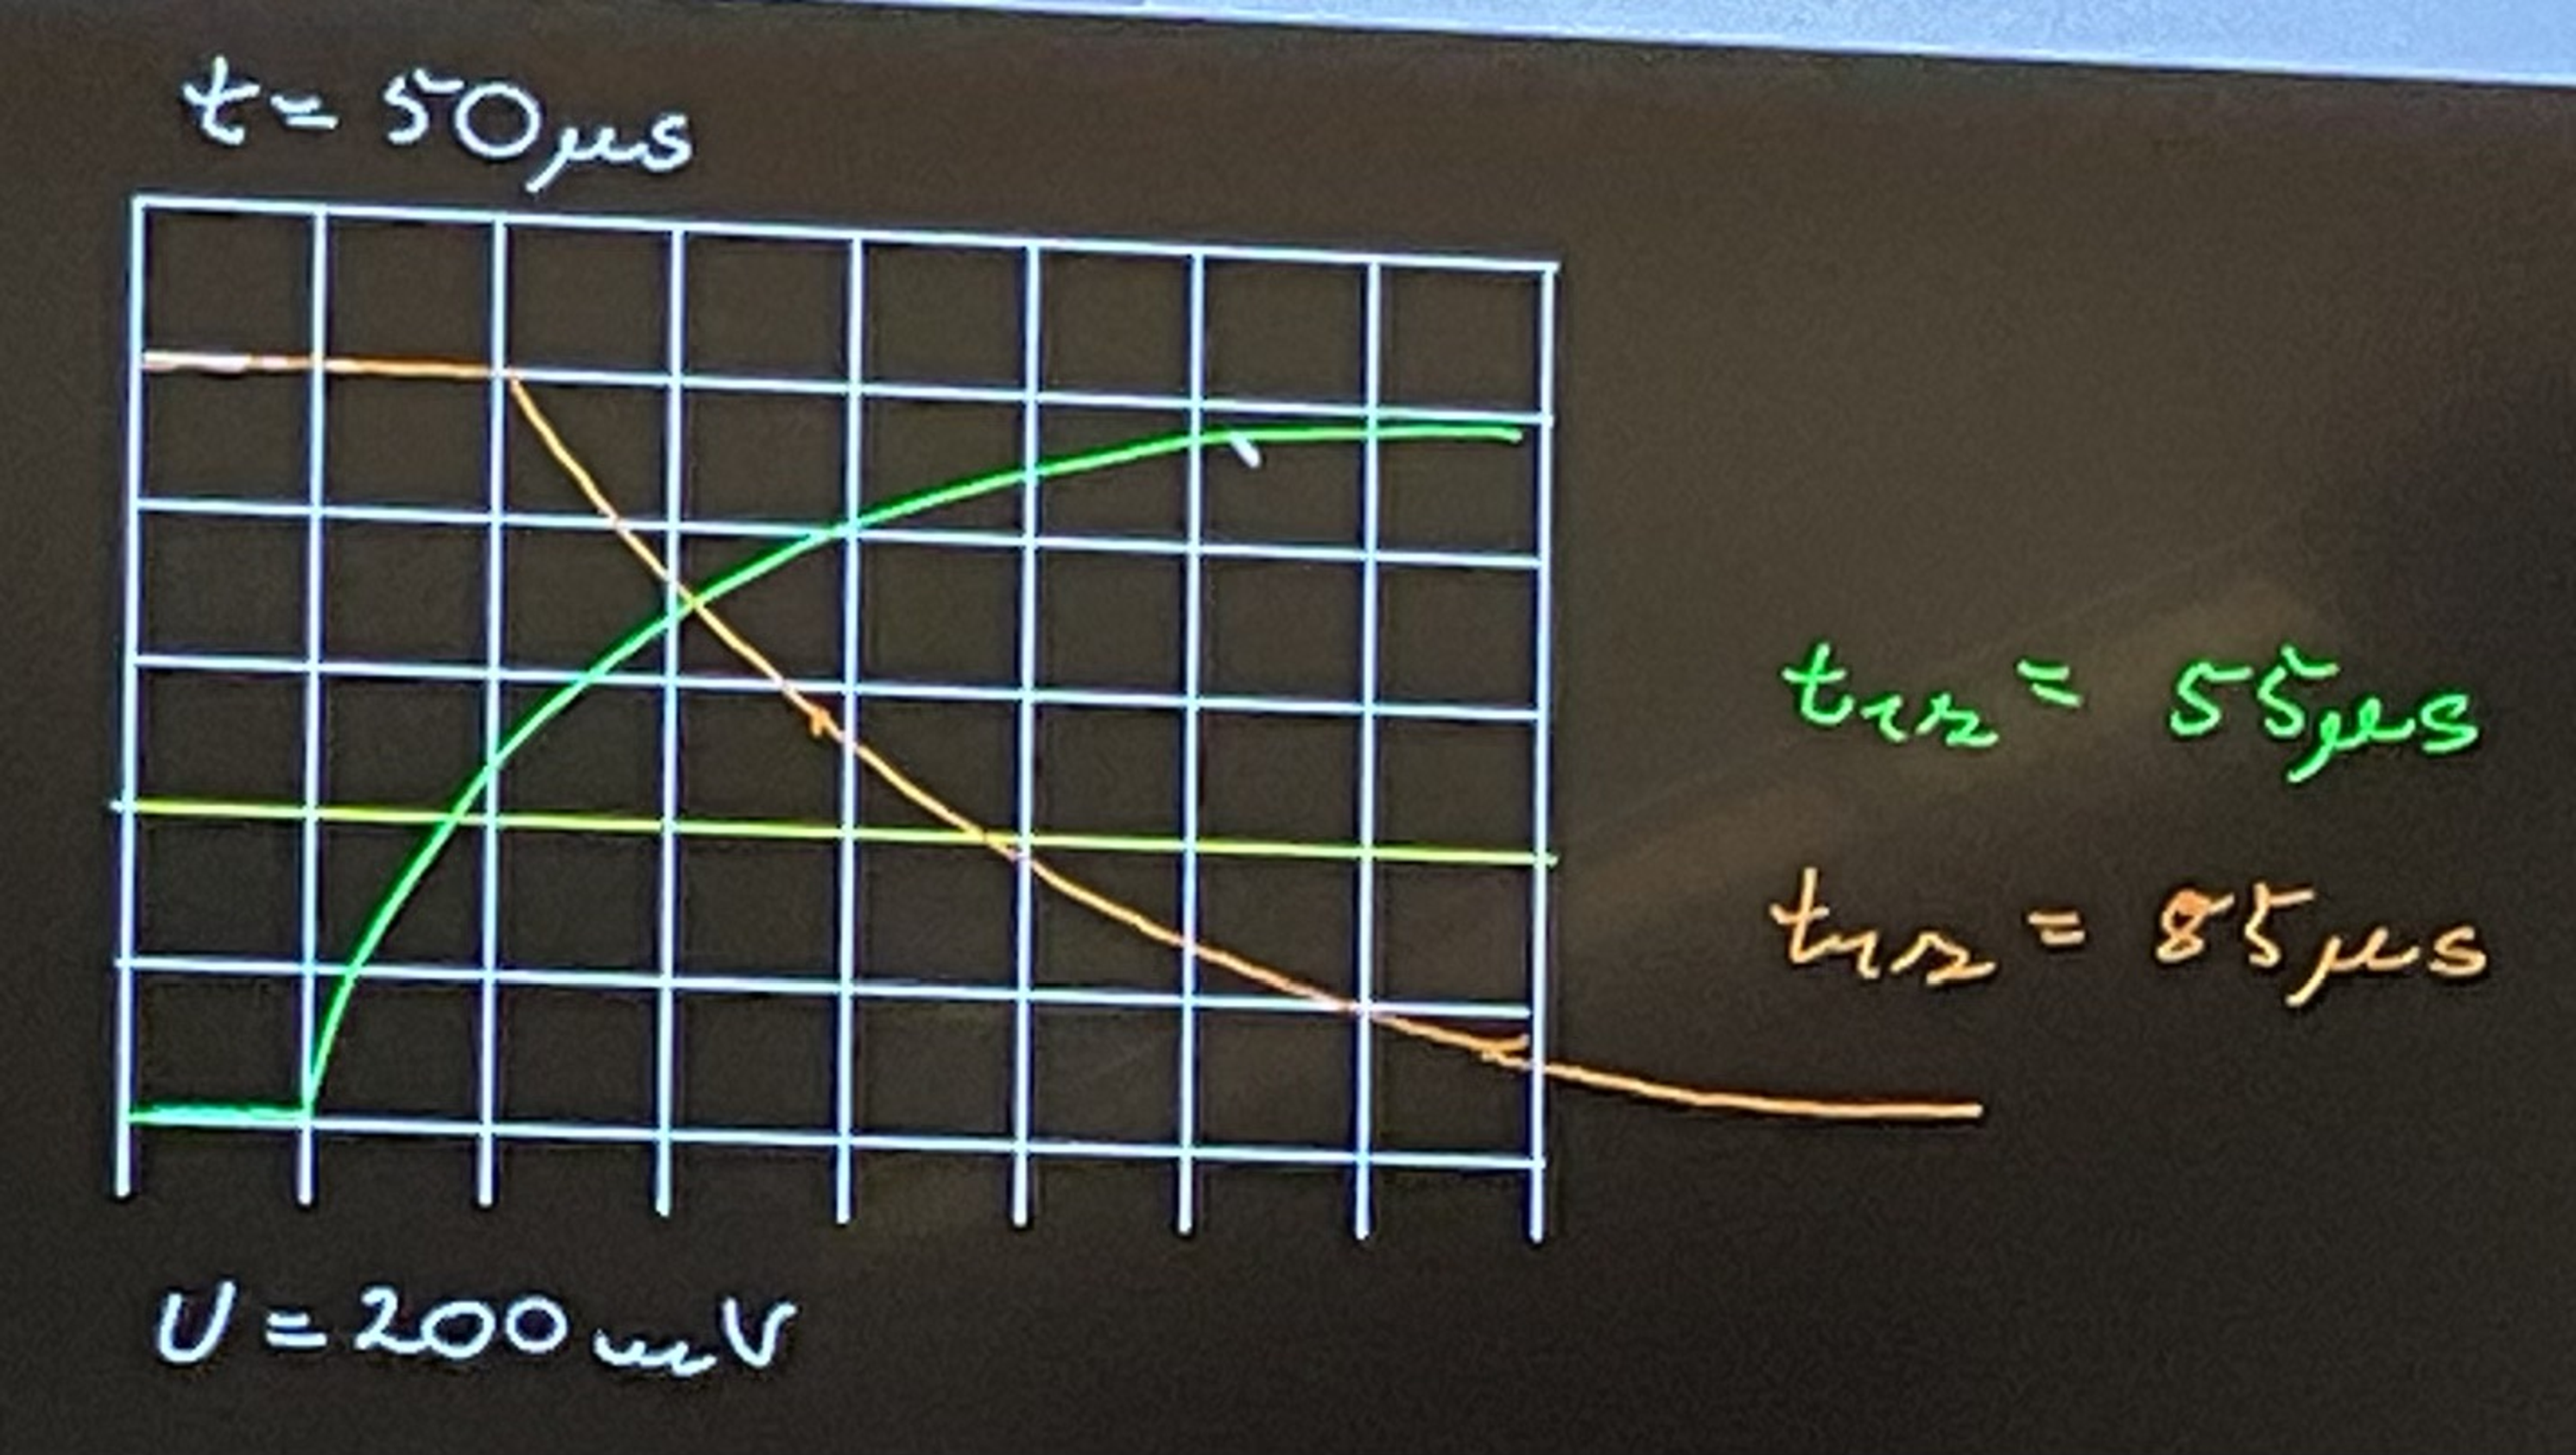
\includegraphics[width=0.7\textwidth]{Images/Ablesen Oszilloskop.pdf}
	\end{center}
	\newpage
	\subsection{Kreisbahn im B-Feld}
	\begin{alignat}{1}
		F_r &= F_L\\
		\frac{m \cdot v^2}{r} &= B \cdot q \cdot v \qquad \mid r \quad \mid : Bqv\\
		r &= \frac{m v}{qB} = \boxed{\frac{m}{q}} \cdot \frac{v}{B}
	\end{alignat}
	
	
	
	
	
	
	
\end{document}
